\setchapterabstract{
    This chapter provides an overview of the most common discrete probability distributions. We start by introducing the Bernoulli distribution, which models a single coin toss. We then move on to the binomial distribution, which models the number of successes in a fixed number of Bernoulli trials. We also introduce the geometric and negative binomial distributions, for the number of trials needed to get the first success and a fixed number of successes, respectively. Finally, we introduce the hypergeometric distribution, which models the number of successes in a sample drawn without replacement from a finite population.
}
\chapter{Discrete Probability Distributions}
\vspace{-1.5cm}


%%%%%%INSERT TOC BELOW 1ST SECTION%%%%%%%%%%%%

{\chaptoc\noindent\begin{minipage}[inner sep=0,outer sep=0]{0.9\linewidth}\section{Bernoulli Distribution}\end{minipage}}

Bernoulli Scheme can describe a series of coin tossing experiments, or the extraction of a ball from an urn with two colors, if there is replacement.

\Definition{
A Bernoulli random variable is a random variable that takes the value $1$ with probability $p$ and the value $0$ with probability $1-p$. We denote a Bernoulli random variable as $X\sim\text{Bern}(p)$. \\
We observe a Bernoulli Scheme when we have:
\begin{itemize}
\item A sequence of $n$ independent trials.
\item Each trial has two possible outcomes: success or failure.
\item The probability of success of a single trial is constant $(p)$.
\end{itemize}
}{Bernoulli Scheme}


\[
x =
\begin{cases}
    0 \quad 1-p\\
    1 \quad p
\end{cases}
\]
\[
X \sim \text{Bern}(p)
\]

What is the expected value, and the variance?
\begin{equation}
\begin{aligned}
    E[X] & = 0 q + 1 p = p \\
    E[X^2] & = 0^2 q + 1^2 p = p \\
    Var[X] & = E[X^2] - E[X]^2 = p - p^2 = p(1-p) = pq
\end{aligned}
\end{equation}

If, in any probability space there is an event, $A$ linked to an indicator function $\mathbbm{1}$, then the indicator function of $A$ is a Bernoulli random variable with parameter $p$.
\[
\mathbbm{1}_A \sim \text{Bern}(p)
\]

\newpage
\section{Binomial Distribution}

\Definition{
The binomial distribution is a discrete probability distribution that models the number of successes in a fixed number of Bernoulli trials.\\
The binomial distribution is characterized by two parameters:
\begin{itemize}
    \item $n$ - the number of trials.
    \item $p$ - the probability of success in each trial.
\end{itemize}
}{Binomial Distribution}

We can define the random variable $X$ as the number of successes in n bernoulli trials, with values $0 \leq k \leq n$. The probability of getting $k$ successes in $n$ trials is given by the binomial distribution.

\[ 
X \sim \text{Bin}(n, p)
\]

The probability distribution function of $X$ is given by\sn{The binomial coefficient $\binom{n}{k}$ is the number of ways to choose $k$ successes in $n$ trials. It is equivalent to writing:
\[
\binom{n}{k} = \frac{n!}{k!(n-k)!}
\]
}
\sn{
\begin{center}
    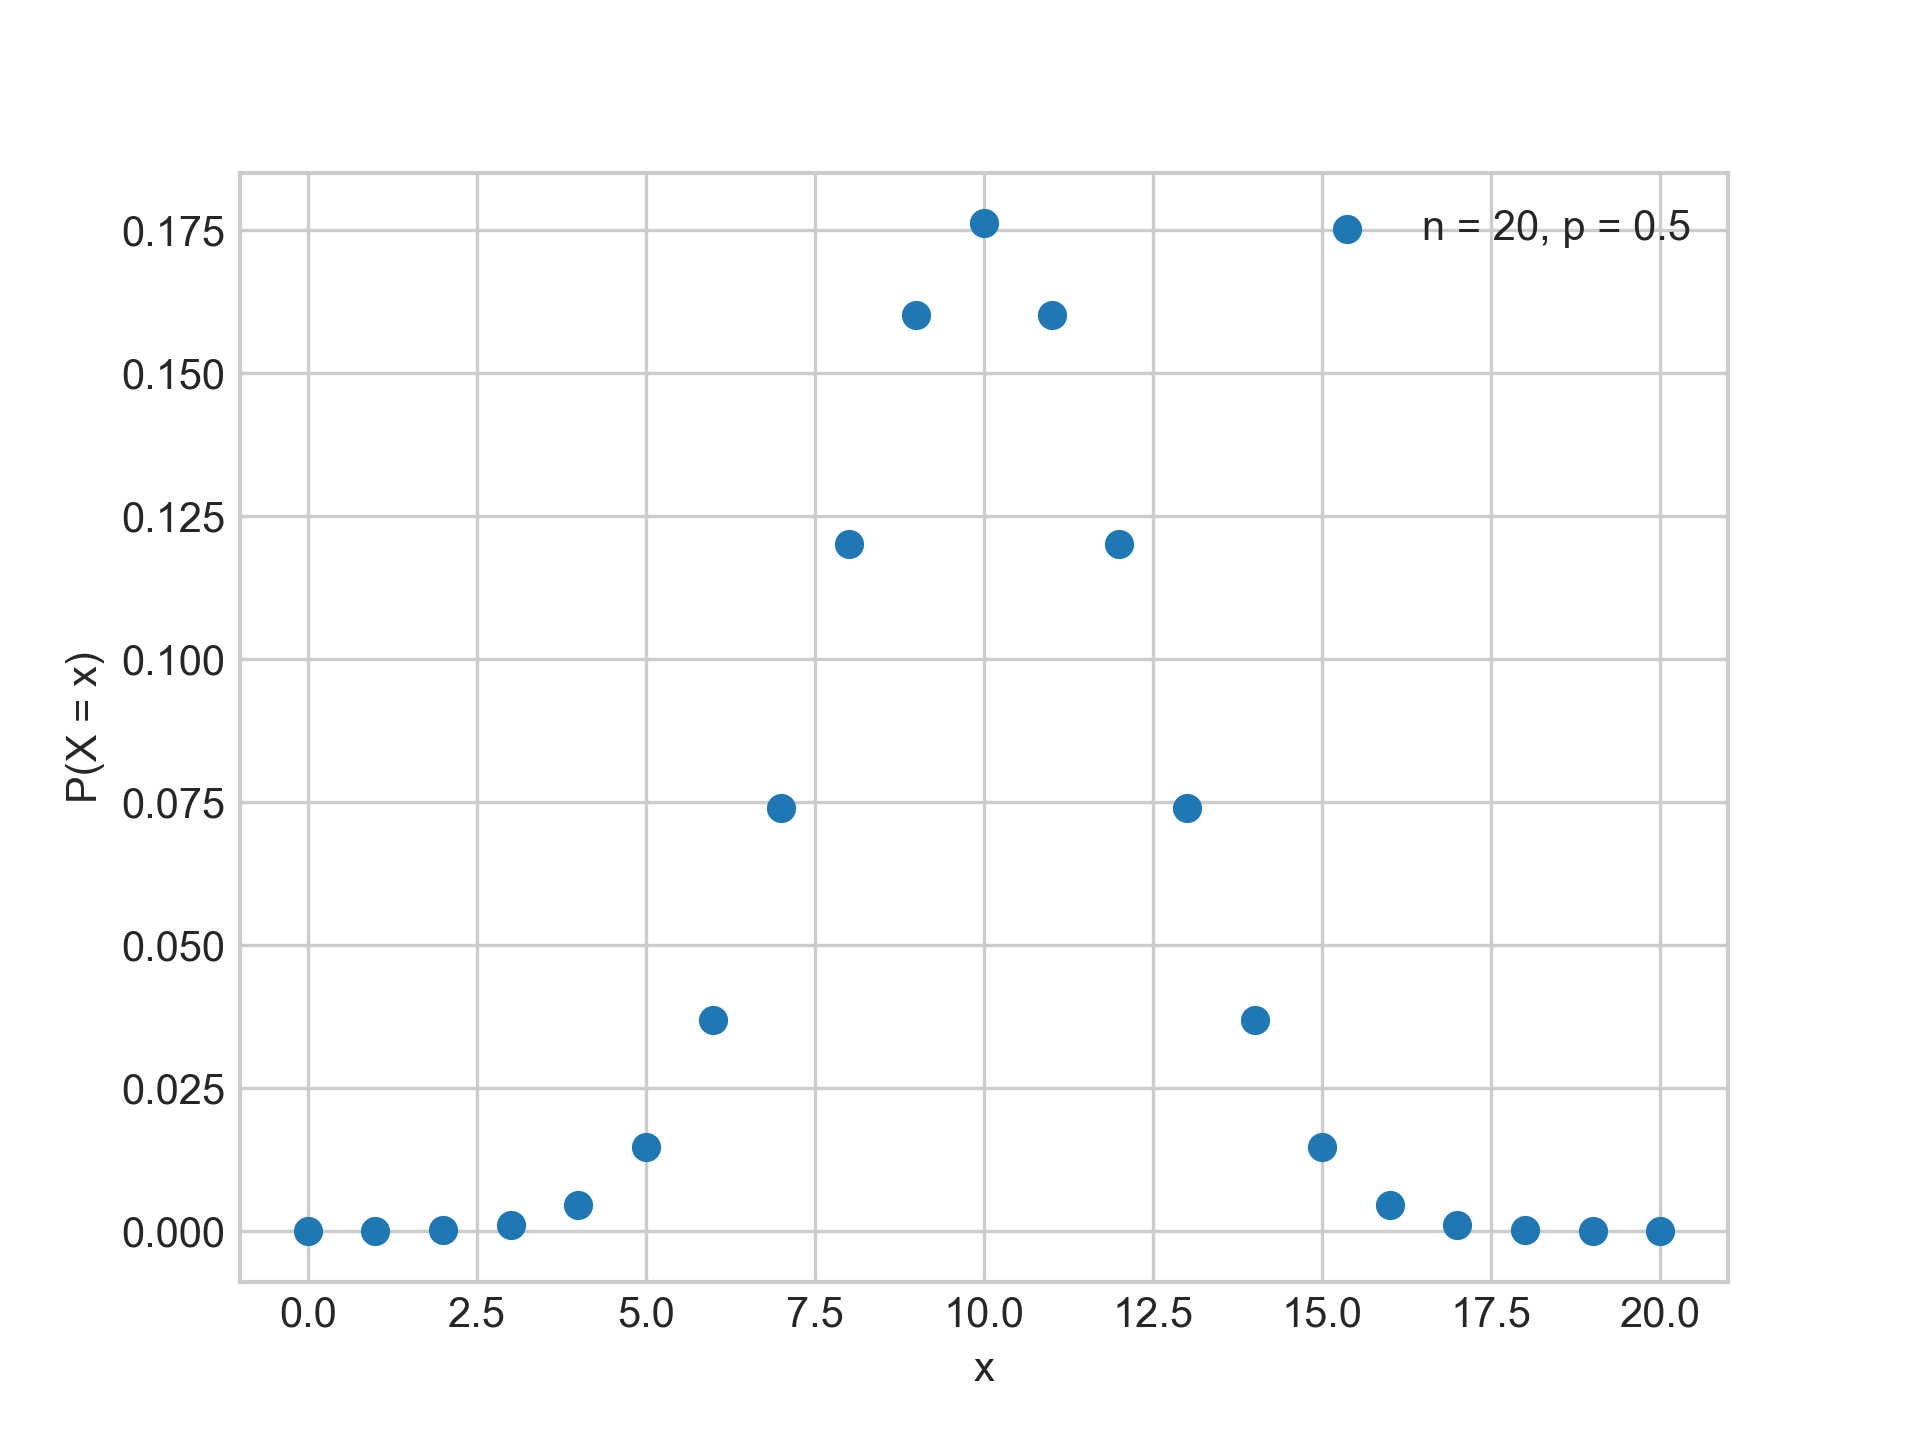
\includegraphics[width=0.4\textwidth]{binomial_pdf.png}
    \captionof{figure}{Probability distribution function of a binomial random variable with p = 0.2 and n = 20.}
    \label{fig:binomial_pdf}
    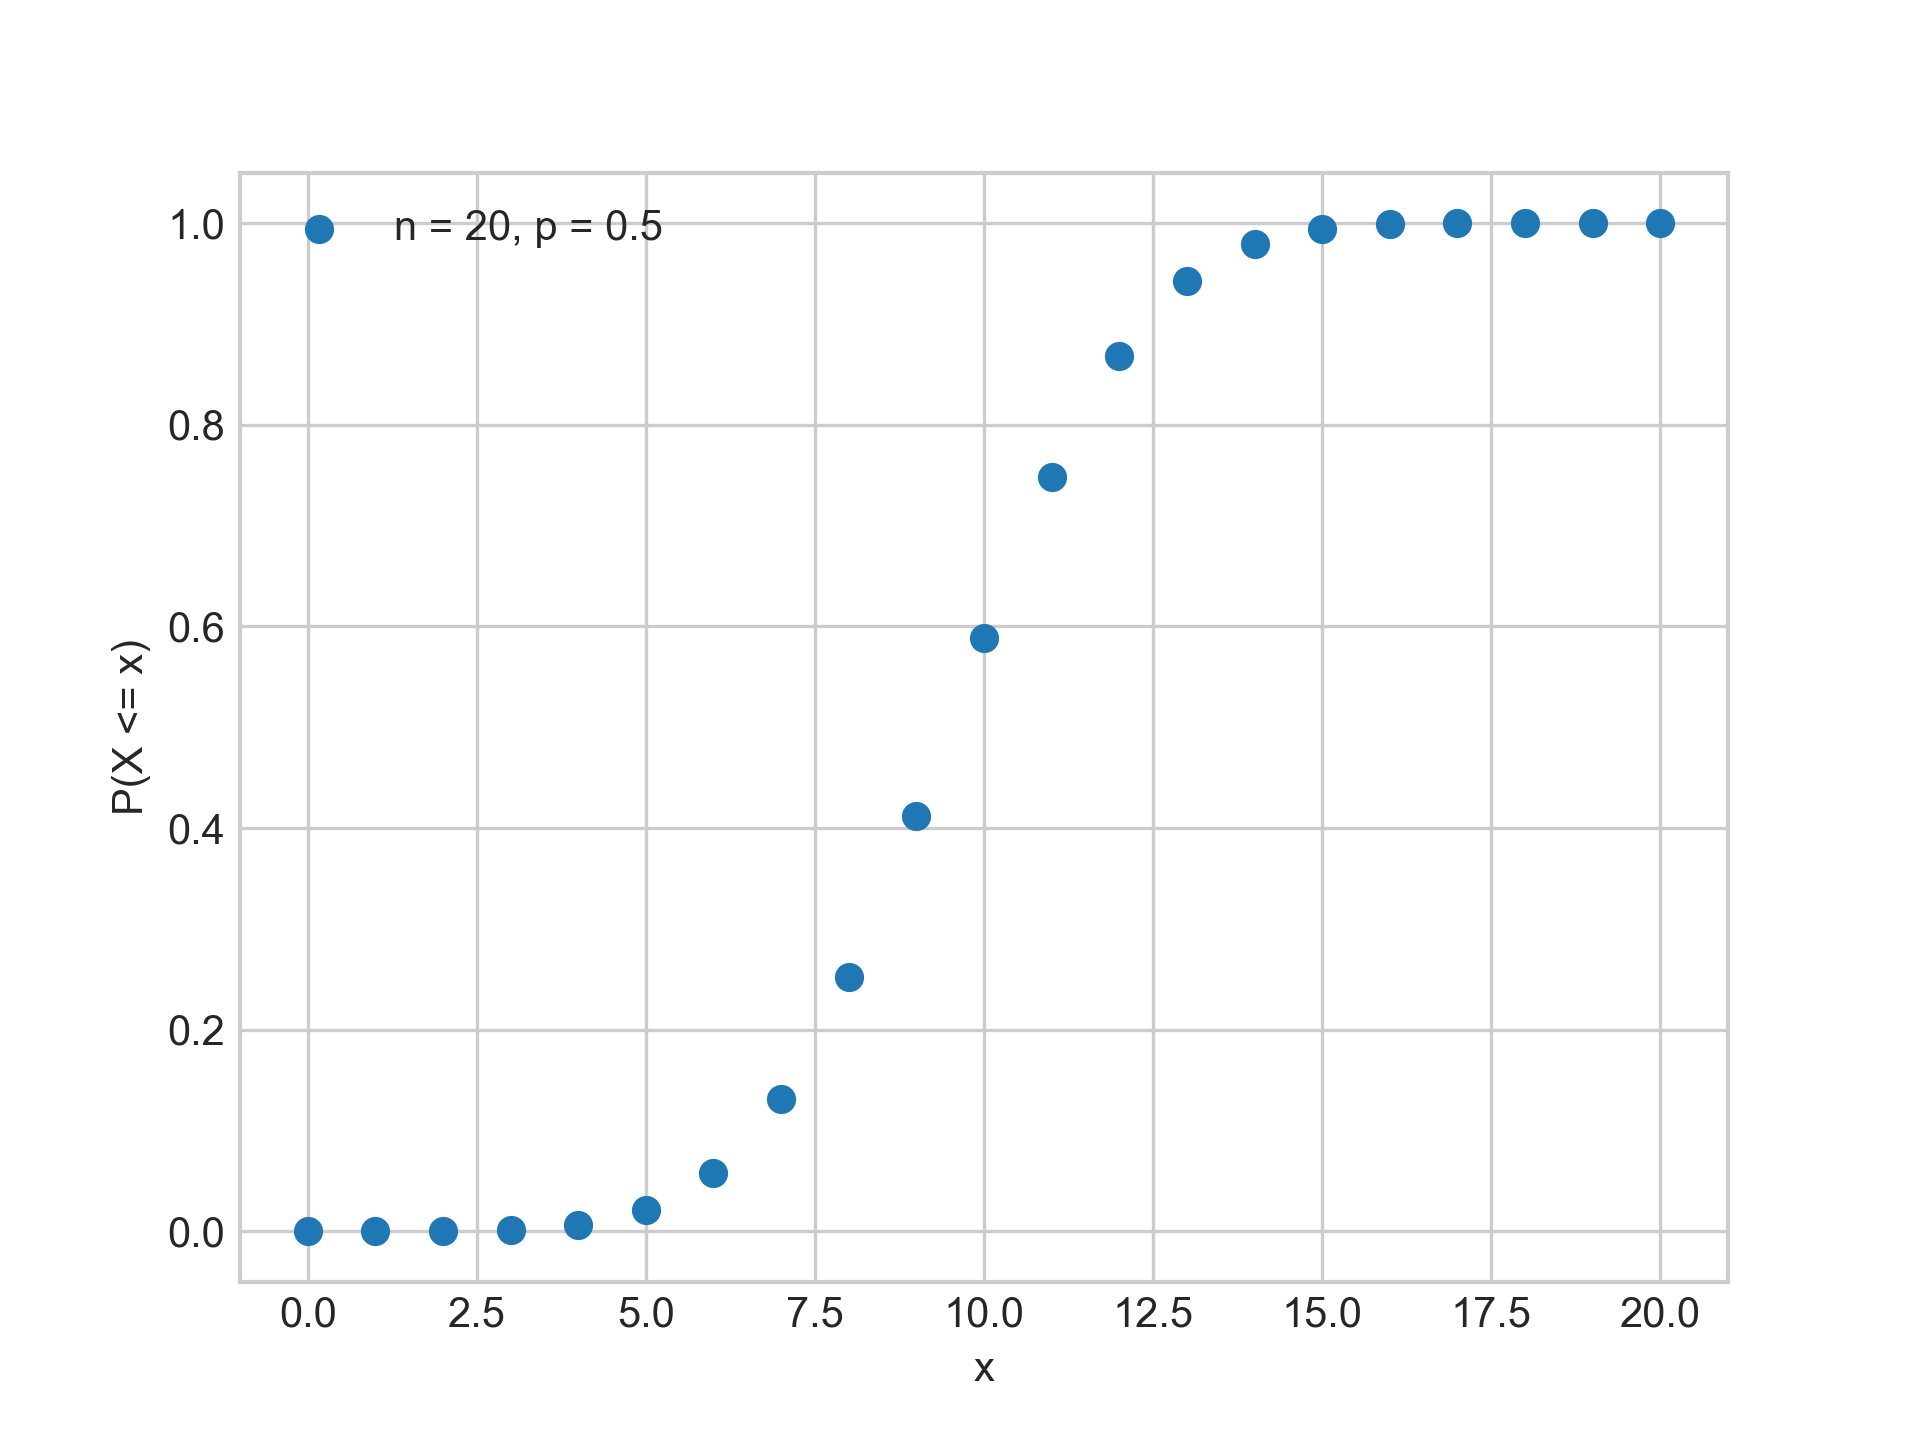
\includegraphics[width=0.4\textwidth]{binomial_cdf.png}
    \captionof{figure}{Cumulative distribution function.}
\end{center}
}:
\begin{equation}
    P(X=k) = \binom{n}{k} p^k q^{n-k}
\end{equation}

\noindent\textbf{What is the link between the binomial and the Bernoulli distribution?}\\
Defining $Y_i$ as the $i^{th}$ Bernoulli random variable, we can say that the sum of $n$ independent Bernoulli random variables is a binomial random variable.
\begin{equation}
    X = \sum_{i=1}^{n} Y_i \sim \text{Bin}(n, p)
\end{equation}

\Example{Adam and Barbara are playing table tennis. In a single game, Barbara wins with probability of $0.6$. If they play a series of $7$ games, what is the probability that Barbara wins exactly $5$ games? Assume that the outcome of each game is independent.}

We can model the number of games Barbara wins as a binomial random variable $X \sim \text{Bin}(7, 0.6)$. The probability of Barbara winning exactly $5$ games is given by:
\[
P(X=5) = \binom{7}{5} 0.6^5 0.4^2
\]

\Example{In the previous setting, what is the probability that Barbara wins at least $5$ games?}

The probability of Barbara winning at least $5$ games is given by:
\[
P(X \geq 5) = P(X=5) + P(X=6) + P(X=7)
\]

\Example{In the previous setting, what is the probability of Barbara winning the last 2 games, given that Barbara won 4 and lost 3 games?}

We need to find the probability that the last two games were wins given that Barbara has 4 wins and 3 losses in total.

The possible scenarios are:
\begin{itemize}
    \item 2 wins, 3 losses in the first 5 games, then 2 wins in the last 2 games.
    \item 3 wins, 2 losses in the first 5 games, then 1 win and 1 loss in the last 2 games.
    \item 4 wins, 1 loss in the first 5 games, then 0 wins in the last 2 games.
\end{itemize}

The only favorable scenario is the first one.

Number of favorable outcomes (2 wins in the last three games): 
$\binom{5}{2} = 10$

Number of possible outcomes: $\binom{7}{4} = 35$

Therefore, the probability is:
\[
P(\text{2 wins in the last 2 games} \mid \text{4 wins and 3 losses}) = \frac{10}{35}
\]

\section{Geometric Distribution}
If $X$ is the number of trials needed to get the first success in a sequence of Bernoulli trials.
\[
P(X=k)
\]

1. For the first success to occur on the \( k \)-th trial, the first \( k-1 \) trials must all result in failures. The probability of failure on each trial is \( 1-p \). Therefore, the probability that the first \( k-1 \) trials all fail is \( (1-p)^{k-1} \).

2. The \( k \)-th trial must be a success. The probability of a success on this trial is \( p \).

Hence, the probability that the first success occurs on the \( k \)-th trial is given by:
\[
P(X = k) = (1-p)^{k-1}p
\]

\Definition{
The geometric distribution is a probability distribution that models the number of Bernoulli trials needed to get the first success.\\
The geometric distribution is characterized by a single parameter:
\begin{itemize}
    \item $p$ - the probability of success in each trial.
\end{itemize}
}{Geometric Distribution}

\[
E[X] = \sum_{k=1}^{+\infty} k(q)^{k-1}p = \frac{1}{p} \qquad Var[X] = \frac{q}{p^2}
\]


\section{Negative Binomial}
If we fix the number of successes desired, and we model the number of trials needed to get the desired number of successes, we get the negative binomial distribution.

\Definition{
The negative binomial distribution is a probability distribution that models the number of Bernoulli trials needed to get a fixed number of successes.\\
The negative binomial distribution is characterized by two parameters:
\begin{itemize}
    \item $n$ - the number of successes desired.
    \item $p$ - the probability of success in each trial.
\end{itemize}
$ X \sim \text{NegBin}(r, p) $
}{Negative Binomial Distribution}

We have $n$ successes in $k$ trials, the number of failures is therefore $k-n$.
Since the last trial must be a success, the number of possible arrangements of outcomes is $\binom{k-1}{n-1}$.
We can then write the probability as:
\[
    P(X=k) = \binom{k-1}{n-1} p^n q^{k-n}
\]

\section{Hypergeometric Distribution}

\Definition{
The hypergeometric distribution is a probability distribution that models the number of successes in a sample of size $n$ drawn without replacement from a finite population of size $N$ that contains $K$ successes.
It is characterized by three parameters:
\begin{itemize}
    \item $N$ - the population size.
    \item $K$ - the number of successes in the population.
    \item $n$ - the sample size.
\end{itemize}
}{Hypergeometric Distribution}

\[
X \sim \text{Hypergeom}(N, K, n)
\]

The probability distribution function of $X$ is given by:
\[
P(X=k) = \frac{\binom{K}{k} \binom{N-K}{n-k}}{\binom{N}{n}}
\]

Its expected value is:
\[
E[X] = n \frac{K}{N}
\]


\setchapterabstract{This chapter is dedicated to continuous probability distributions. We start by introducing the Poisson distribution, which models the number of events occurring in a fixed interval of time or space. We then move on to the exponential distribution, which models the time until the first event occurs in a Poisson process. We also introduce the gamma distribution, which models the sum of $n$ exponential random variables. Finally, we introduce the uniform distribution, which models the probability of all outcomes in an interval being equally likely.}
\chapter{Continuous Probability Distributions}
\vspace{-1.5cm}

{\chaptoc\noindent\begin{minipage}[inner sep=0,outer sep=0]{0.9\linewidth}\section{Poission Distribution}\end{minipage}}

This is the continuous time equivalent of a bernoulli random variable. It is used to model the number of events occurring in an interval of time or space.

An example is the number of phone calls received by a person. At any given time, the number of calls received is either zero or one, modeled by a Poisson distribution.

Fixing the time interval $[0, T]$, $X =\text{ number of events in }[0, T]$ is a Poisson random variable\sn{
    \begin{center}
        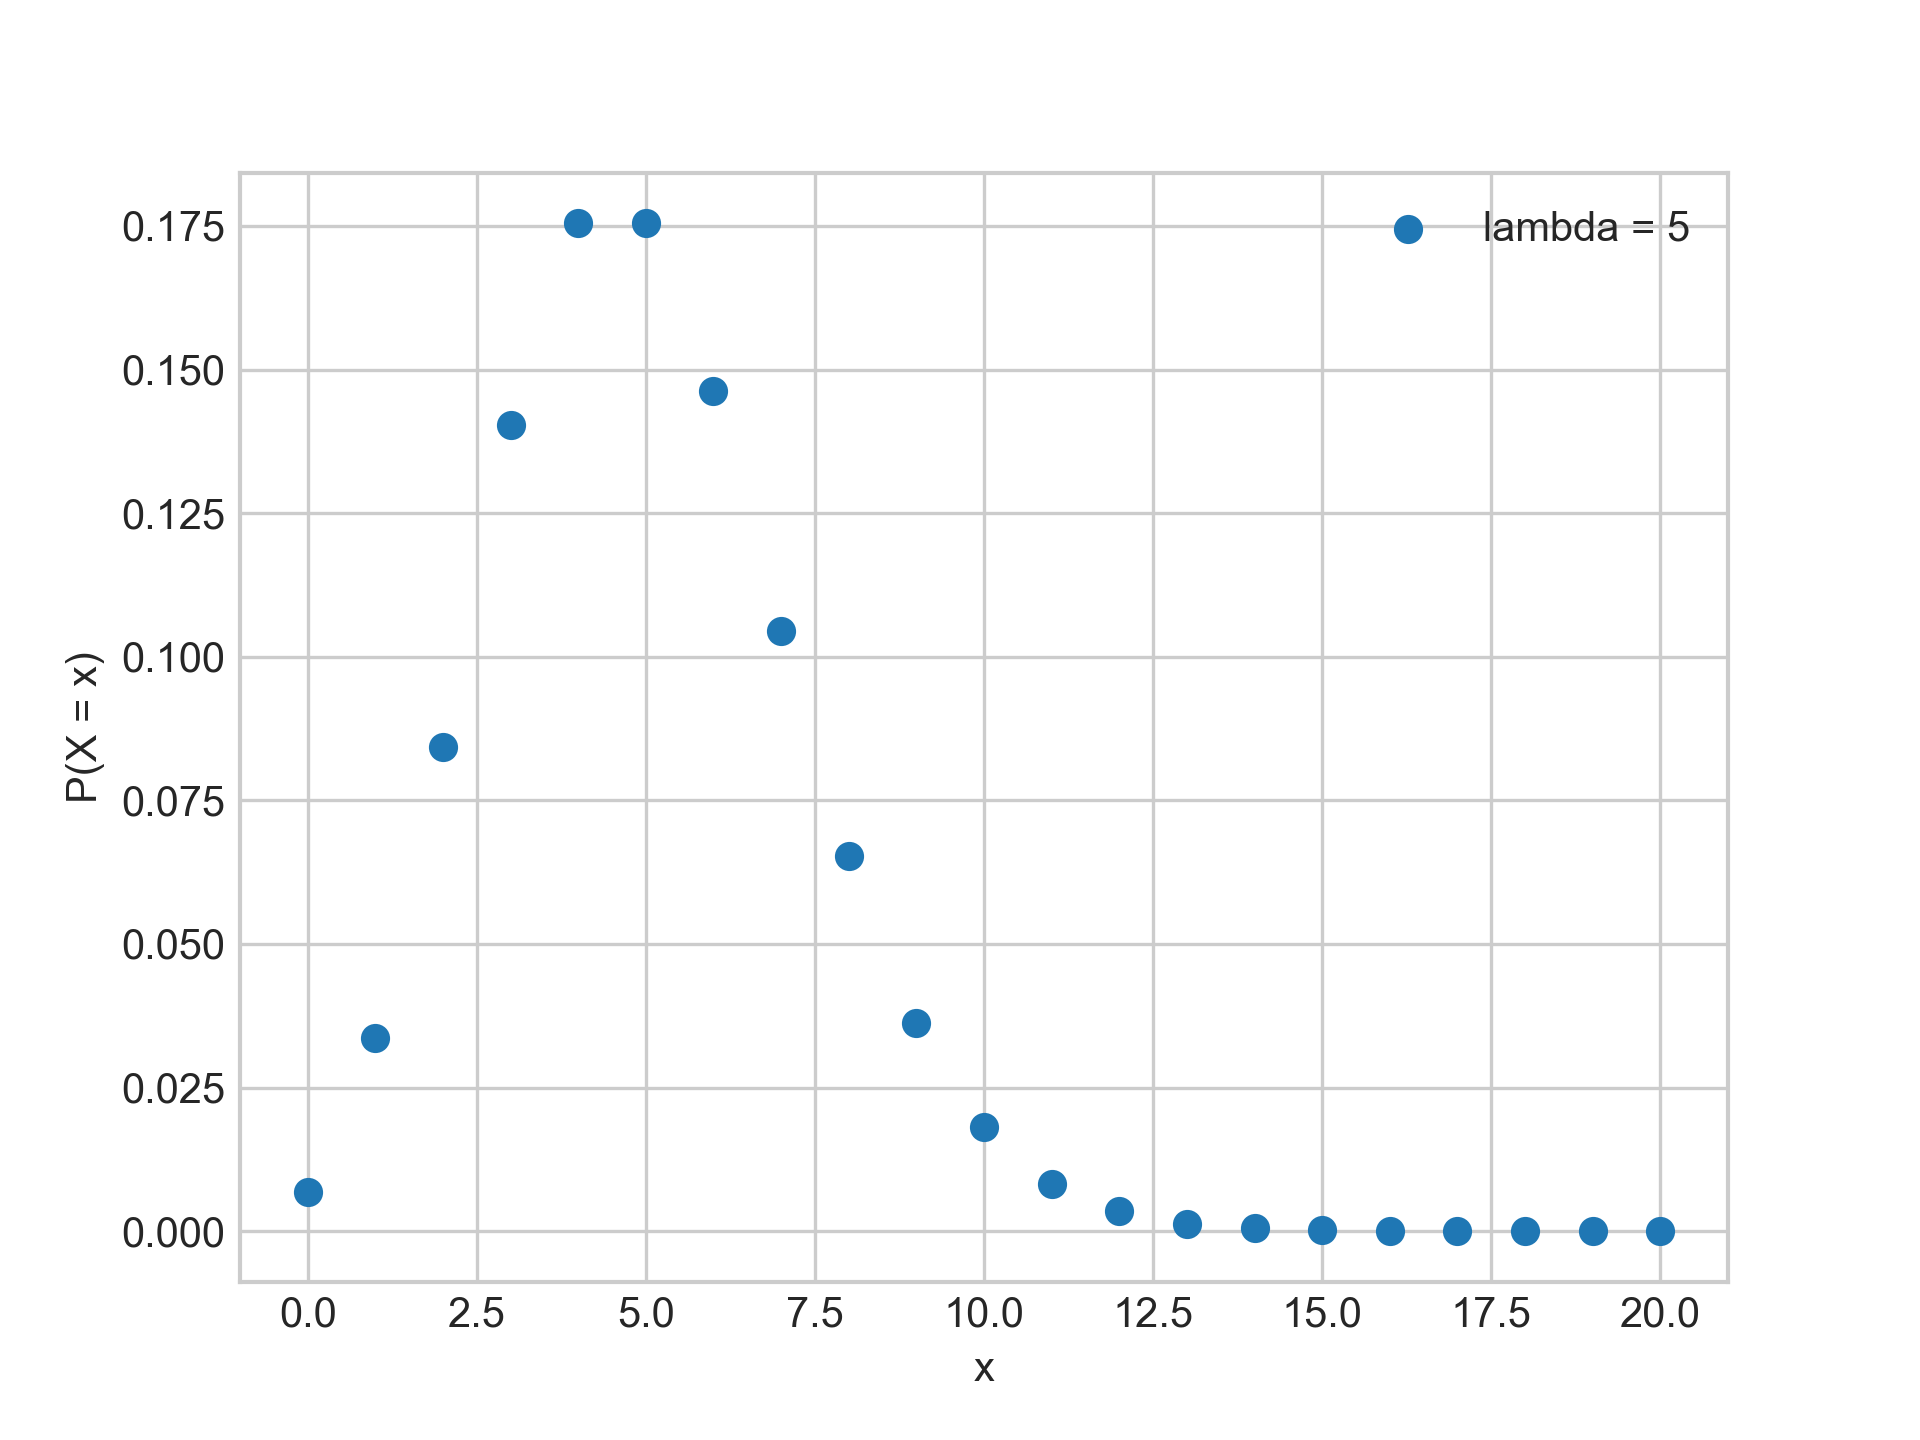
\includegraphics[width=0.4\textwidth]{poisson_pdf.png}
        \captionof{figure}{Probability distribution function of a Poisson random variable with $\lambda = 5$.}
        \label{fig:poisson_pdf}
        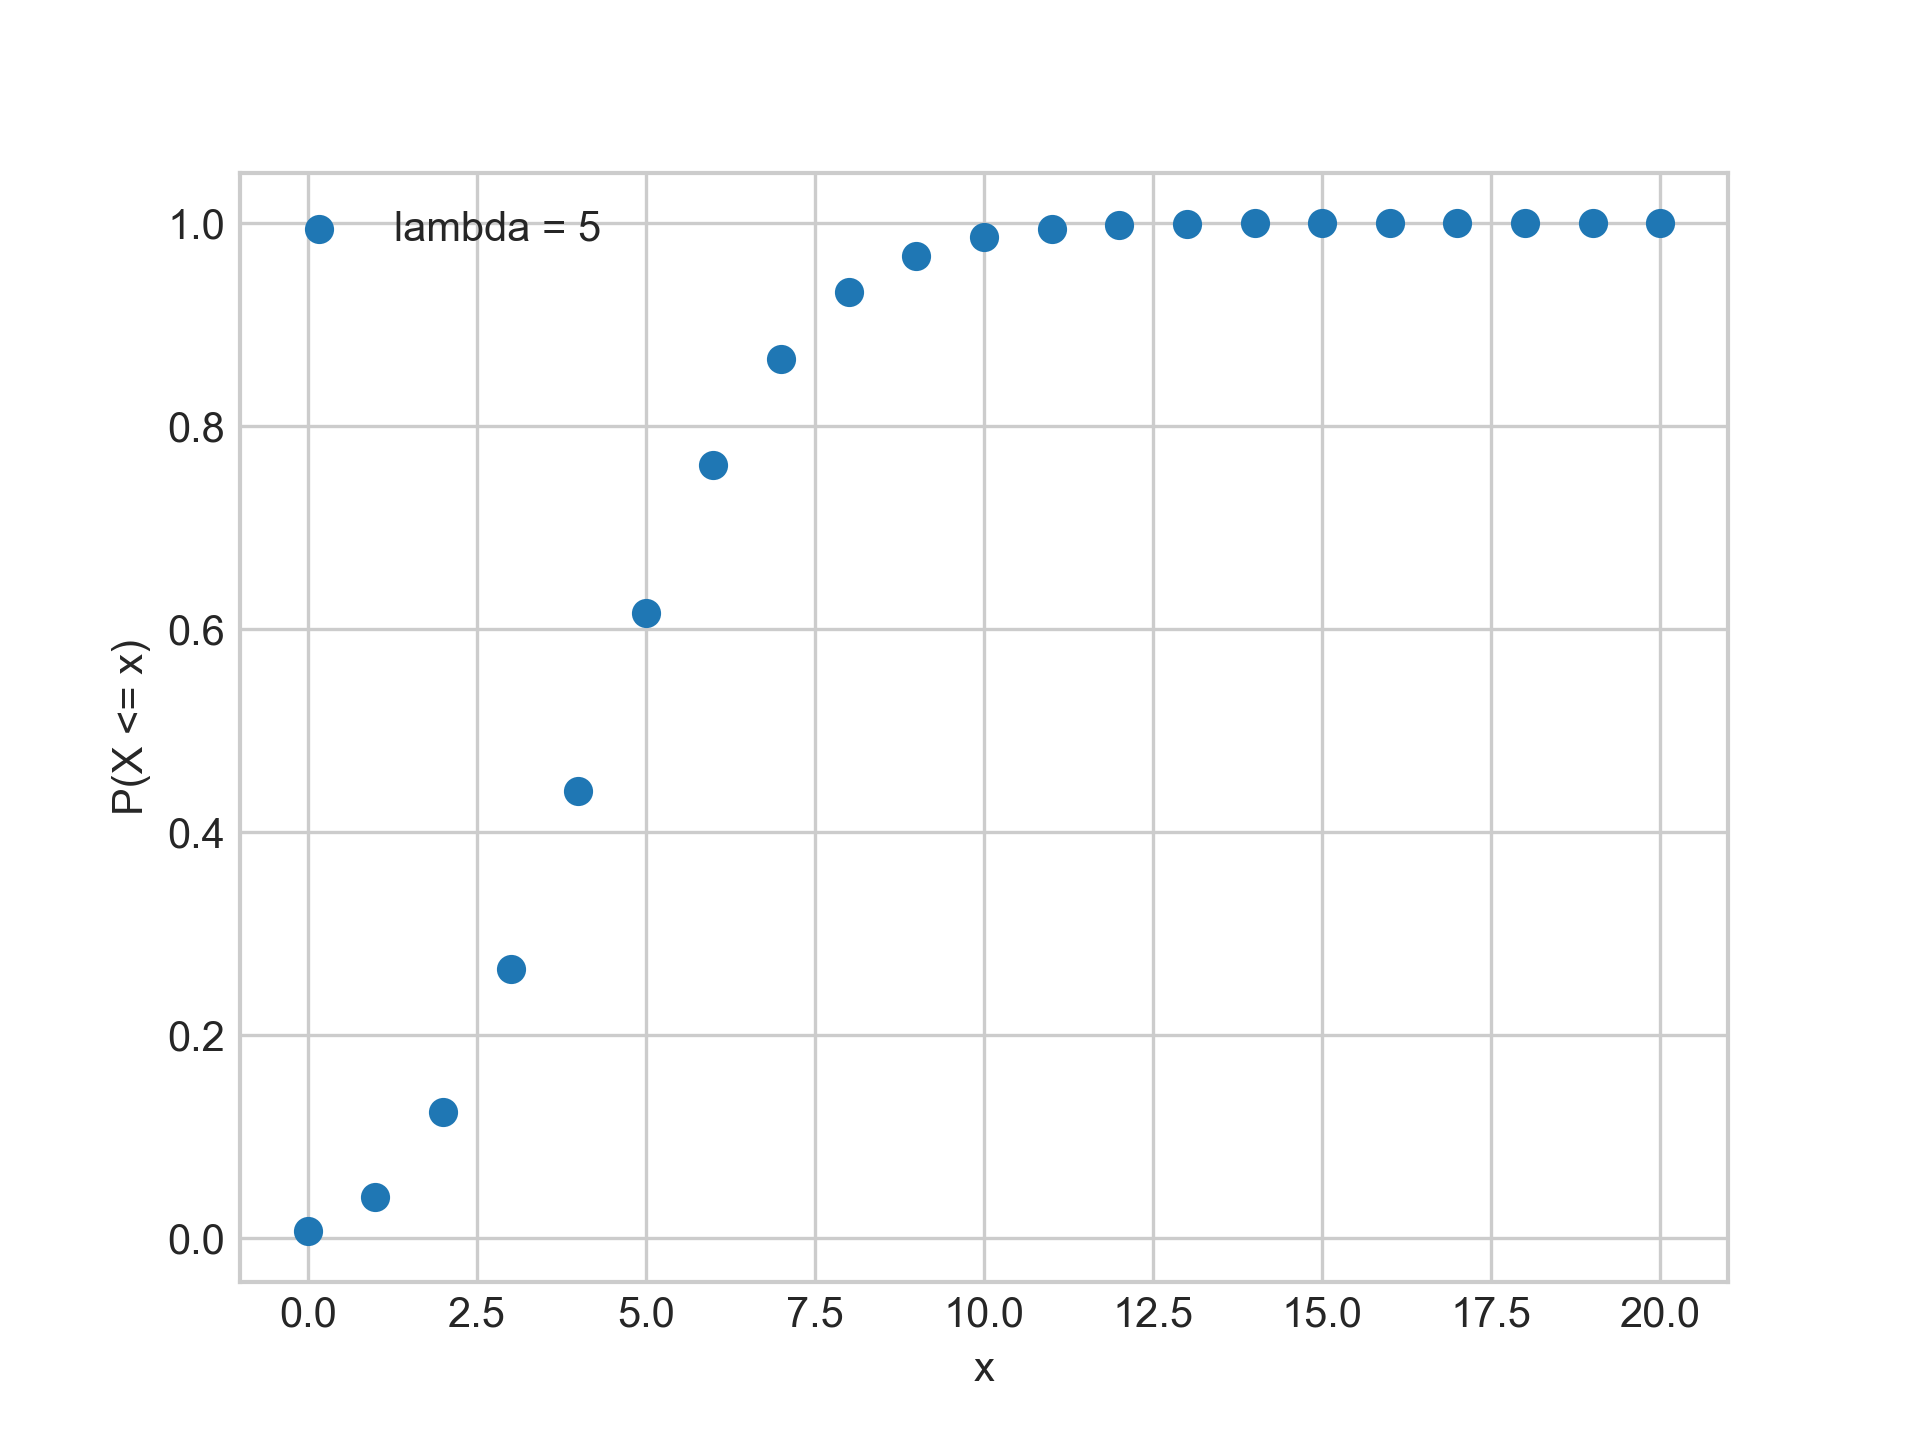
\includegraphics[width=0.4\textwidth]{poisson_cdf.png}
        \captionof{figure}{Cumulative distribution function.}
    \end{center}
}.

\Definition{
The Poisson distribution is a probability distribution that models the number of events occurring in a fixed interval of time or space.\\
The Poisson distribution is characterized by a single parameter:
\begin{itemize}
    \item $\lambda$ - the average rate of events occurring in the interval
    \[\lambda = \frac{\text{number of arrivals}}{\text{time interval}}\]
\end{itemize}
}{Poisson Distribution}

The probability of having 1 arrival in a time interval is given by:
\[
P(X=1) \approx \lambda \Delta t 
\]
\[
P(X=1) = \lambda \Delta t + o(\Delta t)
\]

The probability distribution function of a Poisson random variable is given by:
\[
P(X=k) = \frac{e^{-\lambda T} (\lambda T)^k}{k!}
\]

\section{Exponential Distribution}

If $X$ is the waiting time until the first event occurs in a Poisson process, then $X$ is an exponential random variable

\Definition{
The exponential distribution is a probability distribution that models the time until the first event occurs in a Poisson process.\\
The exponential distribution is characterized by a single parameter:
\begin{itemize}
    \item $\lambda$ - the rate of events occurring in the Poisson process.
\end{itemize}
}{Exponential Distribution}

The probability distribution function of an exponential random variable is given by \sn{
    \begin{center}
        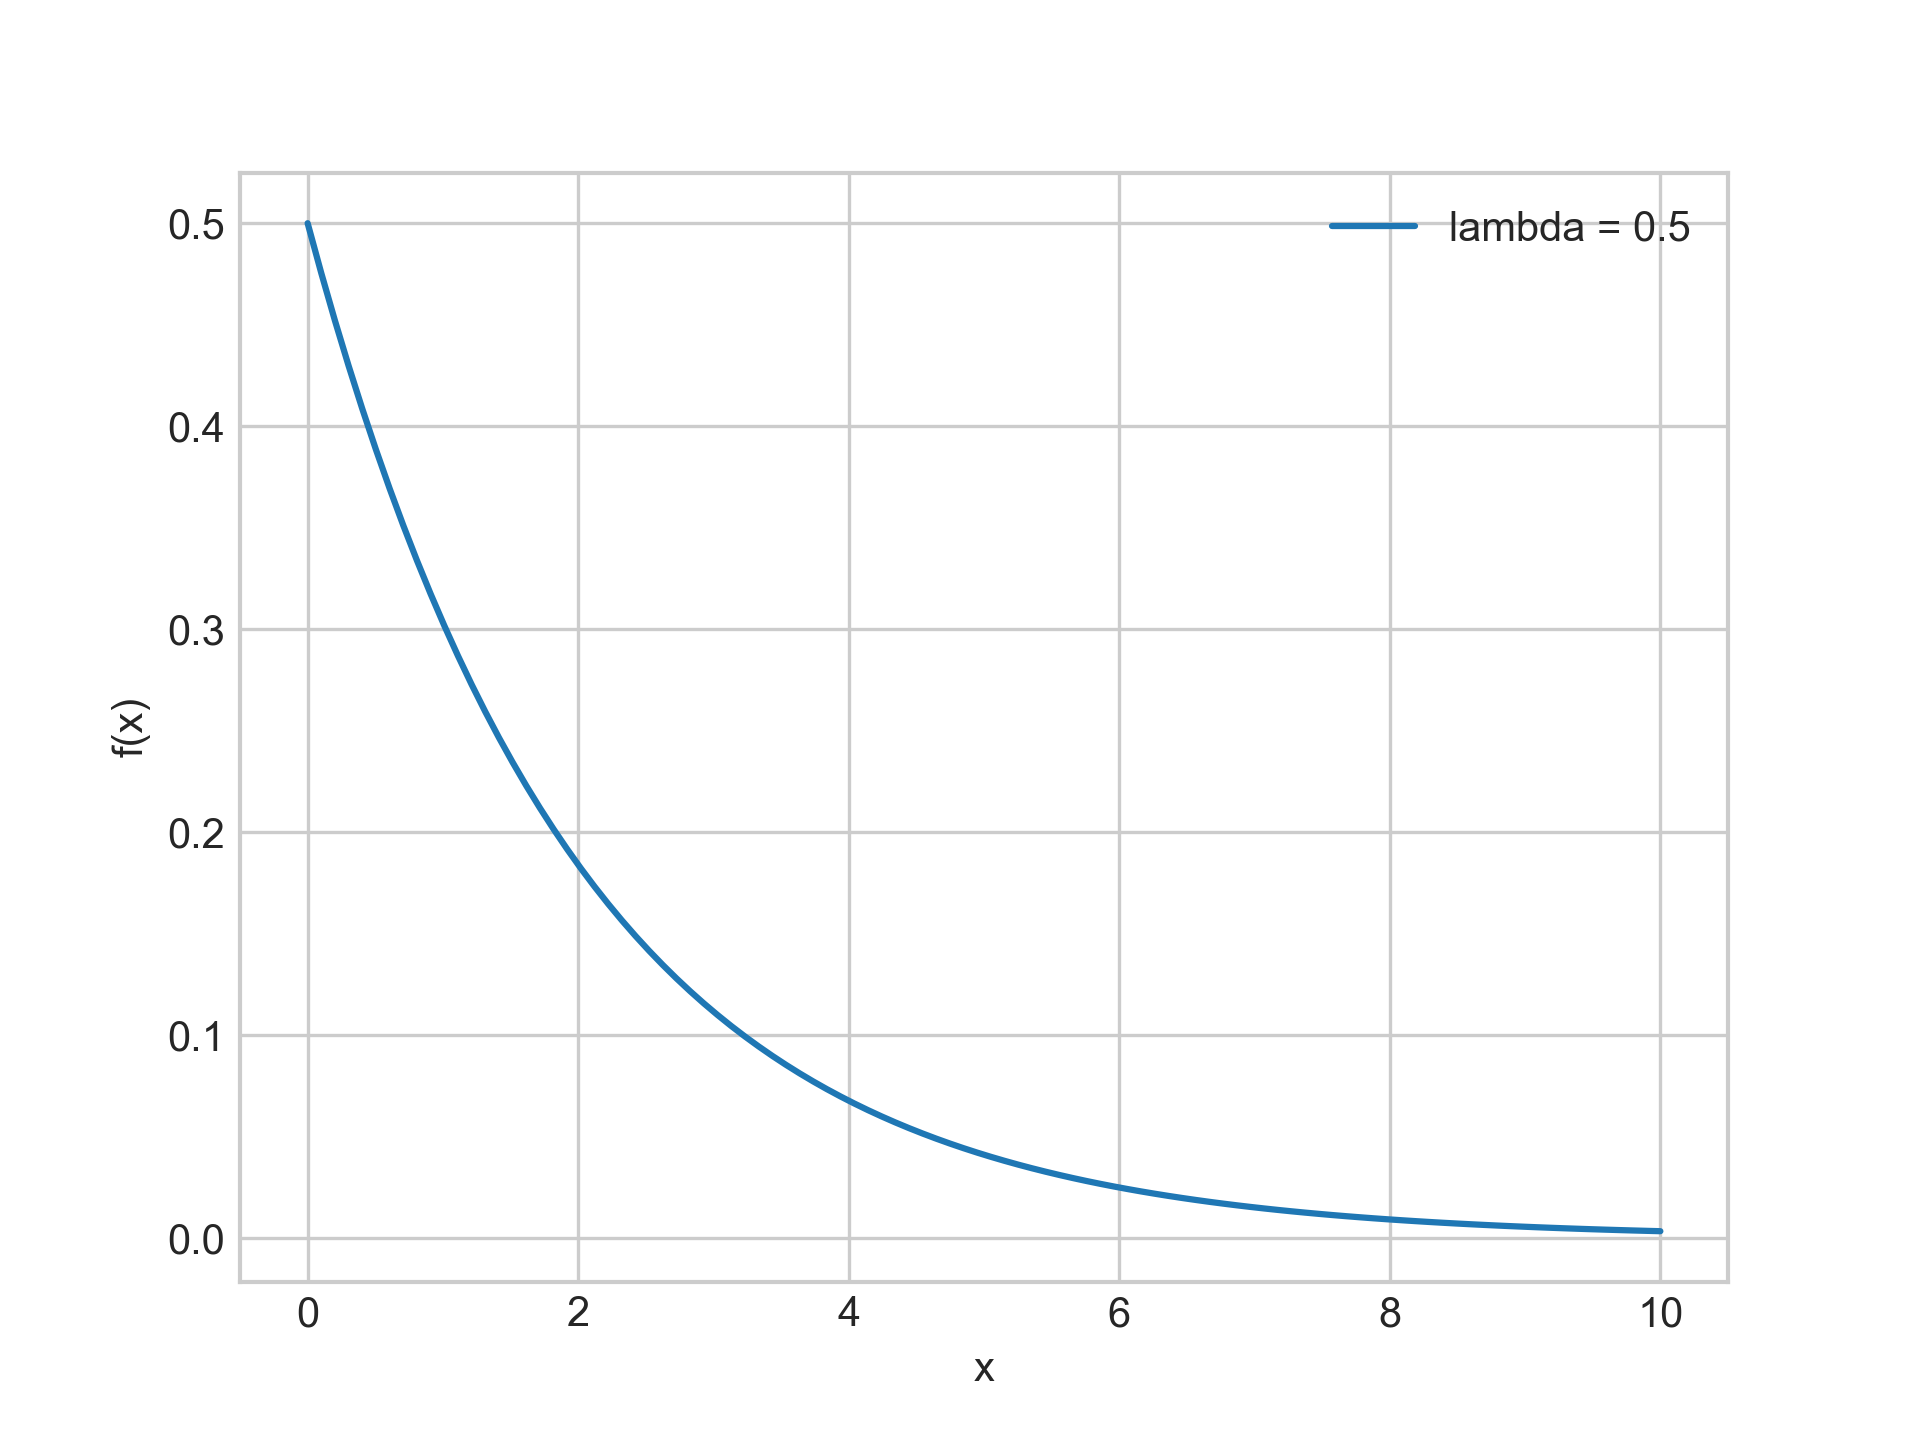
\includegraphics[width=0.4\textwidth]{exponential_pdf.png}
        \captionof{figure}{Probability distribution function of an exponential random variable with $\lambda = 0.5$.}
        \label{fig:exponential_pdf}
        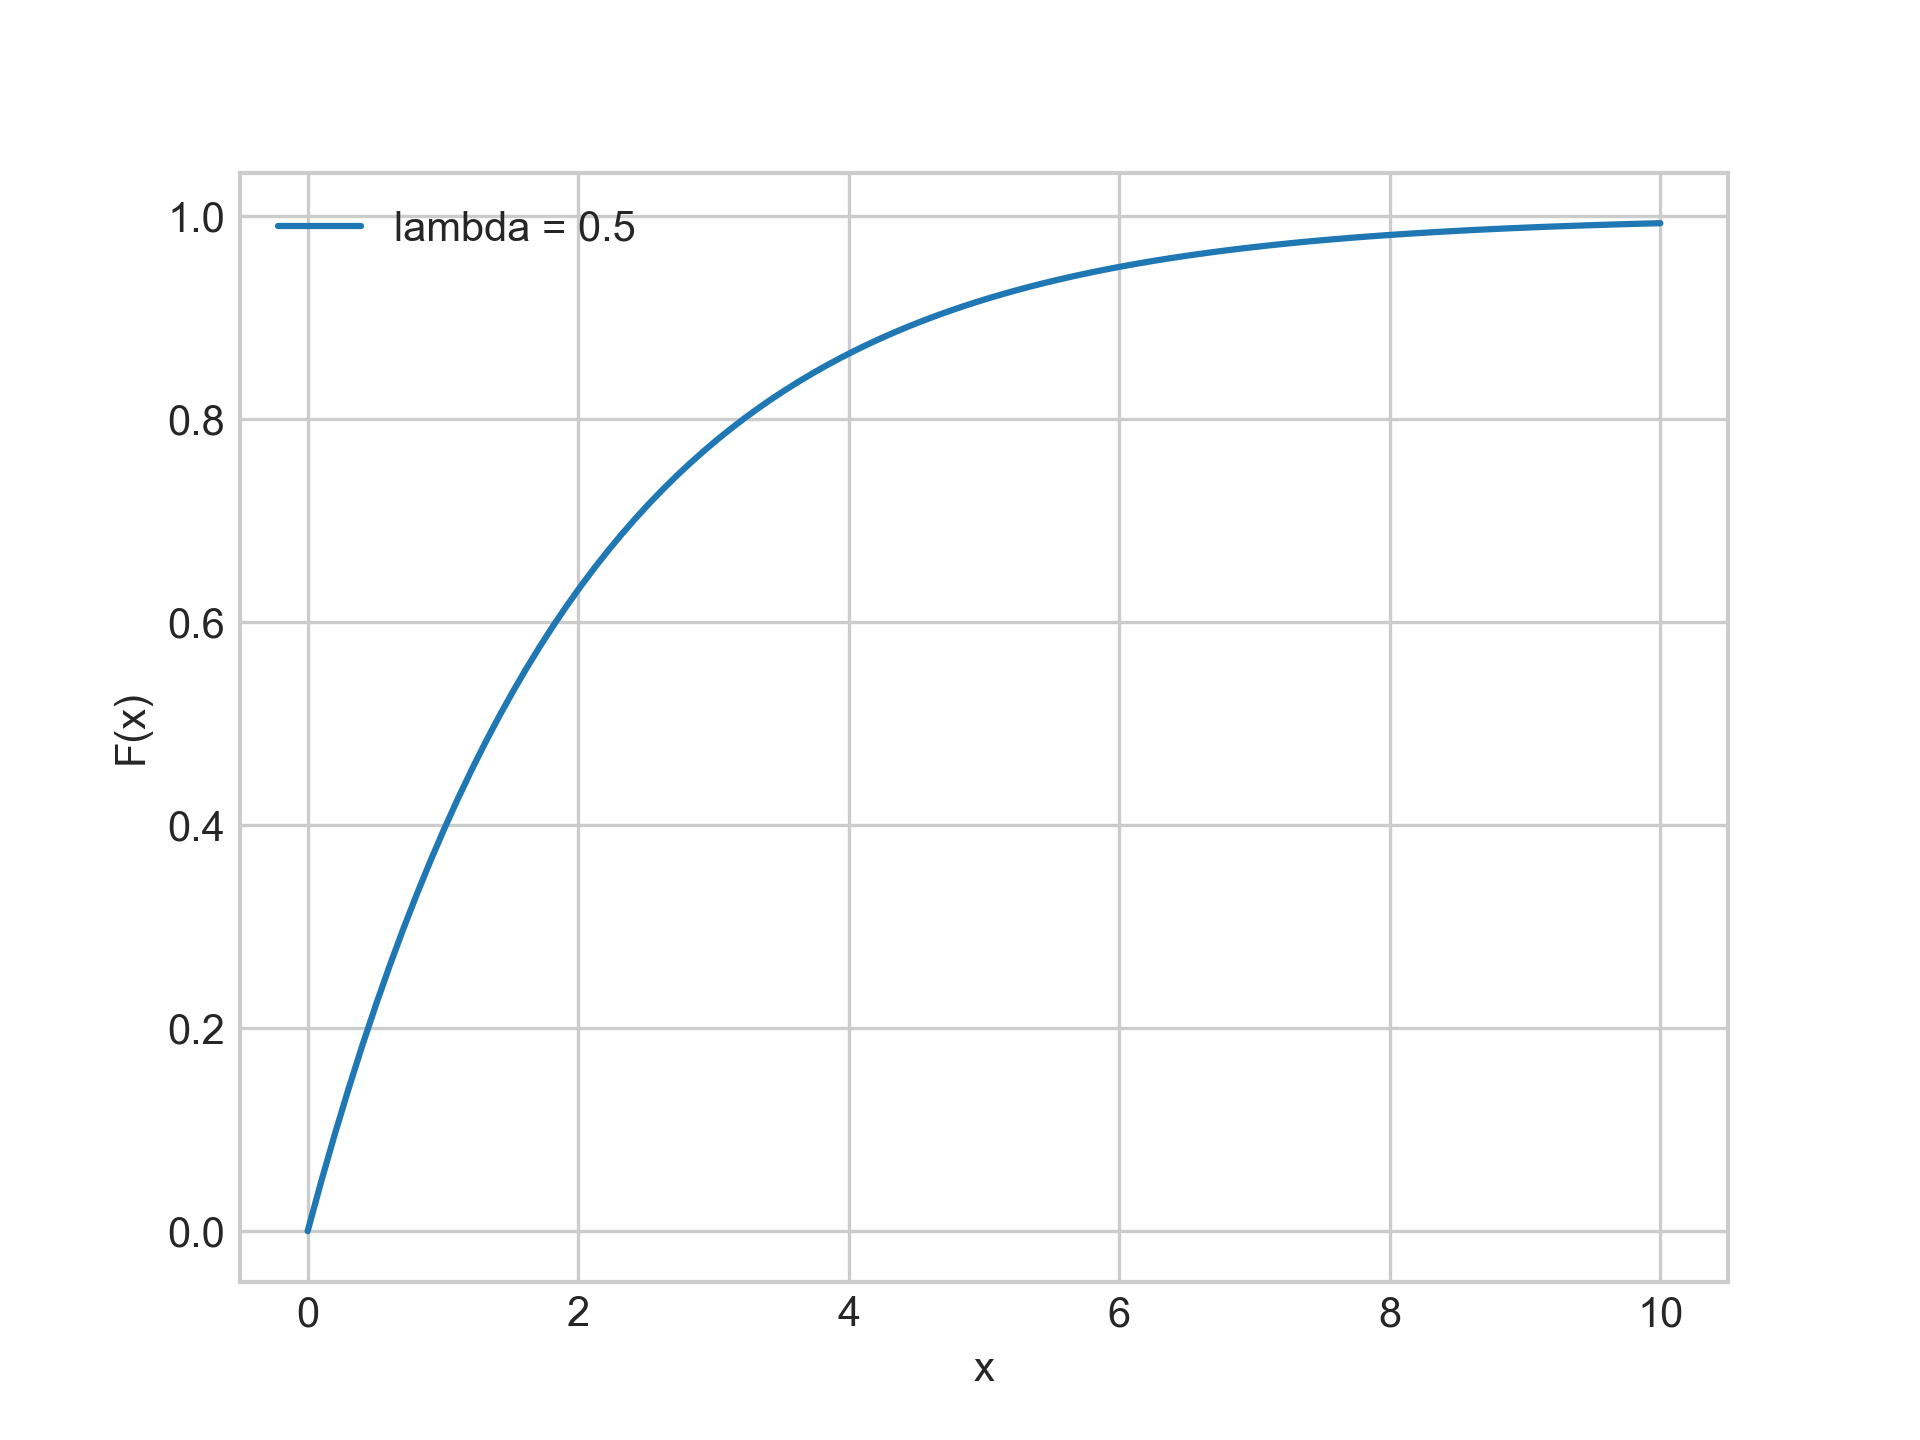
\includegraphics[width=0.4\textwidth]{exponential_cdf.png}
        \captionof{figure}{Cumulative distribution function.}
    \end{center}
}:
\[
f(x) = 
\begin{cases}
    \lambda e^{-\lambda x} & x \geq 0 \\
    0 & x < 0
\end{cases}
\]

The expected value and variance of an exponential random variable are given by:
\[
E[T] = \int_{0}^{+\infty} x f(x) dx = \frac{1}{\lambda} \qquad Var[T] = \frac{1}{\lambda^2}
\]

The exponential distribution is memoryless, meaning that the probability of an event occurring in the next interval (waiting time) is independent of the time that has already passed.


\section{Gamma Distribution}
\Definition{
The gamma function is defined as:\\
\[
\Gamma(z) = \int_{0}^{+\infty} x^{z-1} e^{-x} dx
\]
It is defined as long as the exponent $z$ is positive.
}{Gamma Function}


Properties of the gamma function:
\begin{itemize}
    \item $\Gamma(z+1) = z\Gamma(z)$
    \item $\Gamma(1) = 1$
    \item $\Gamma(n+1) = n!$
\end{itemize}

The most important property of the gamma function is its recursive definition\sn{
    Integration by part:
    \[
    \int u dv = uv - \int v du
    \]
}:
\Proposition{
\[ \Gamma(z+1) = z\Gamma(z) \]
}{
    \begin{equation}
        \begin{aligned}
            \Gamma(z+1) & = \int_{0}^{+\infty} x^z e^{-x} dx \\
            & = \left[-x^z e^{-x}\right]_{0}^{+\infty} + z\int_{0}^{+\infty} x^{z-1} e^{-x} dx = z\Gamma(z)
        \end{aligned}
        \end{equation}
}

From this property, we can see that the gamma function is a generalization of the factorial function. For any positive integer $n$, we have $\Gamma(n+1) = n!$.

Starting from the gamma function, we can define the gamma distribution\sn{
    \begin{center}
        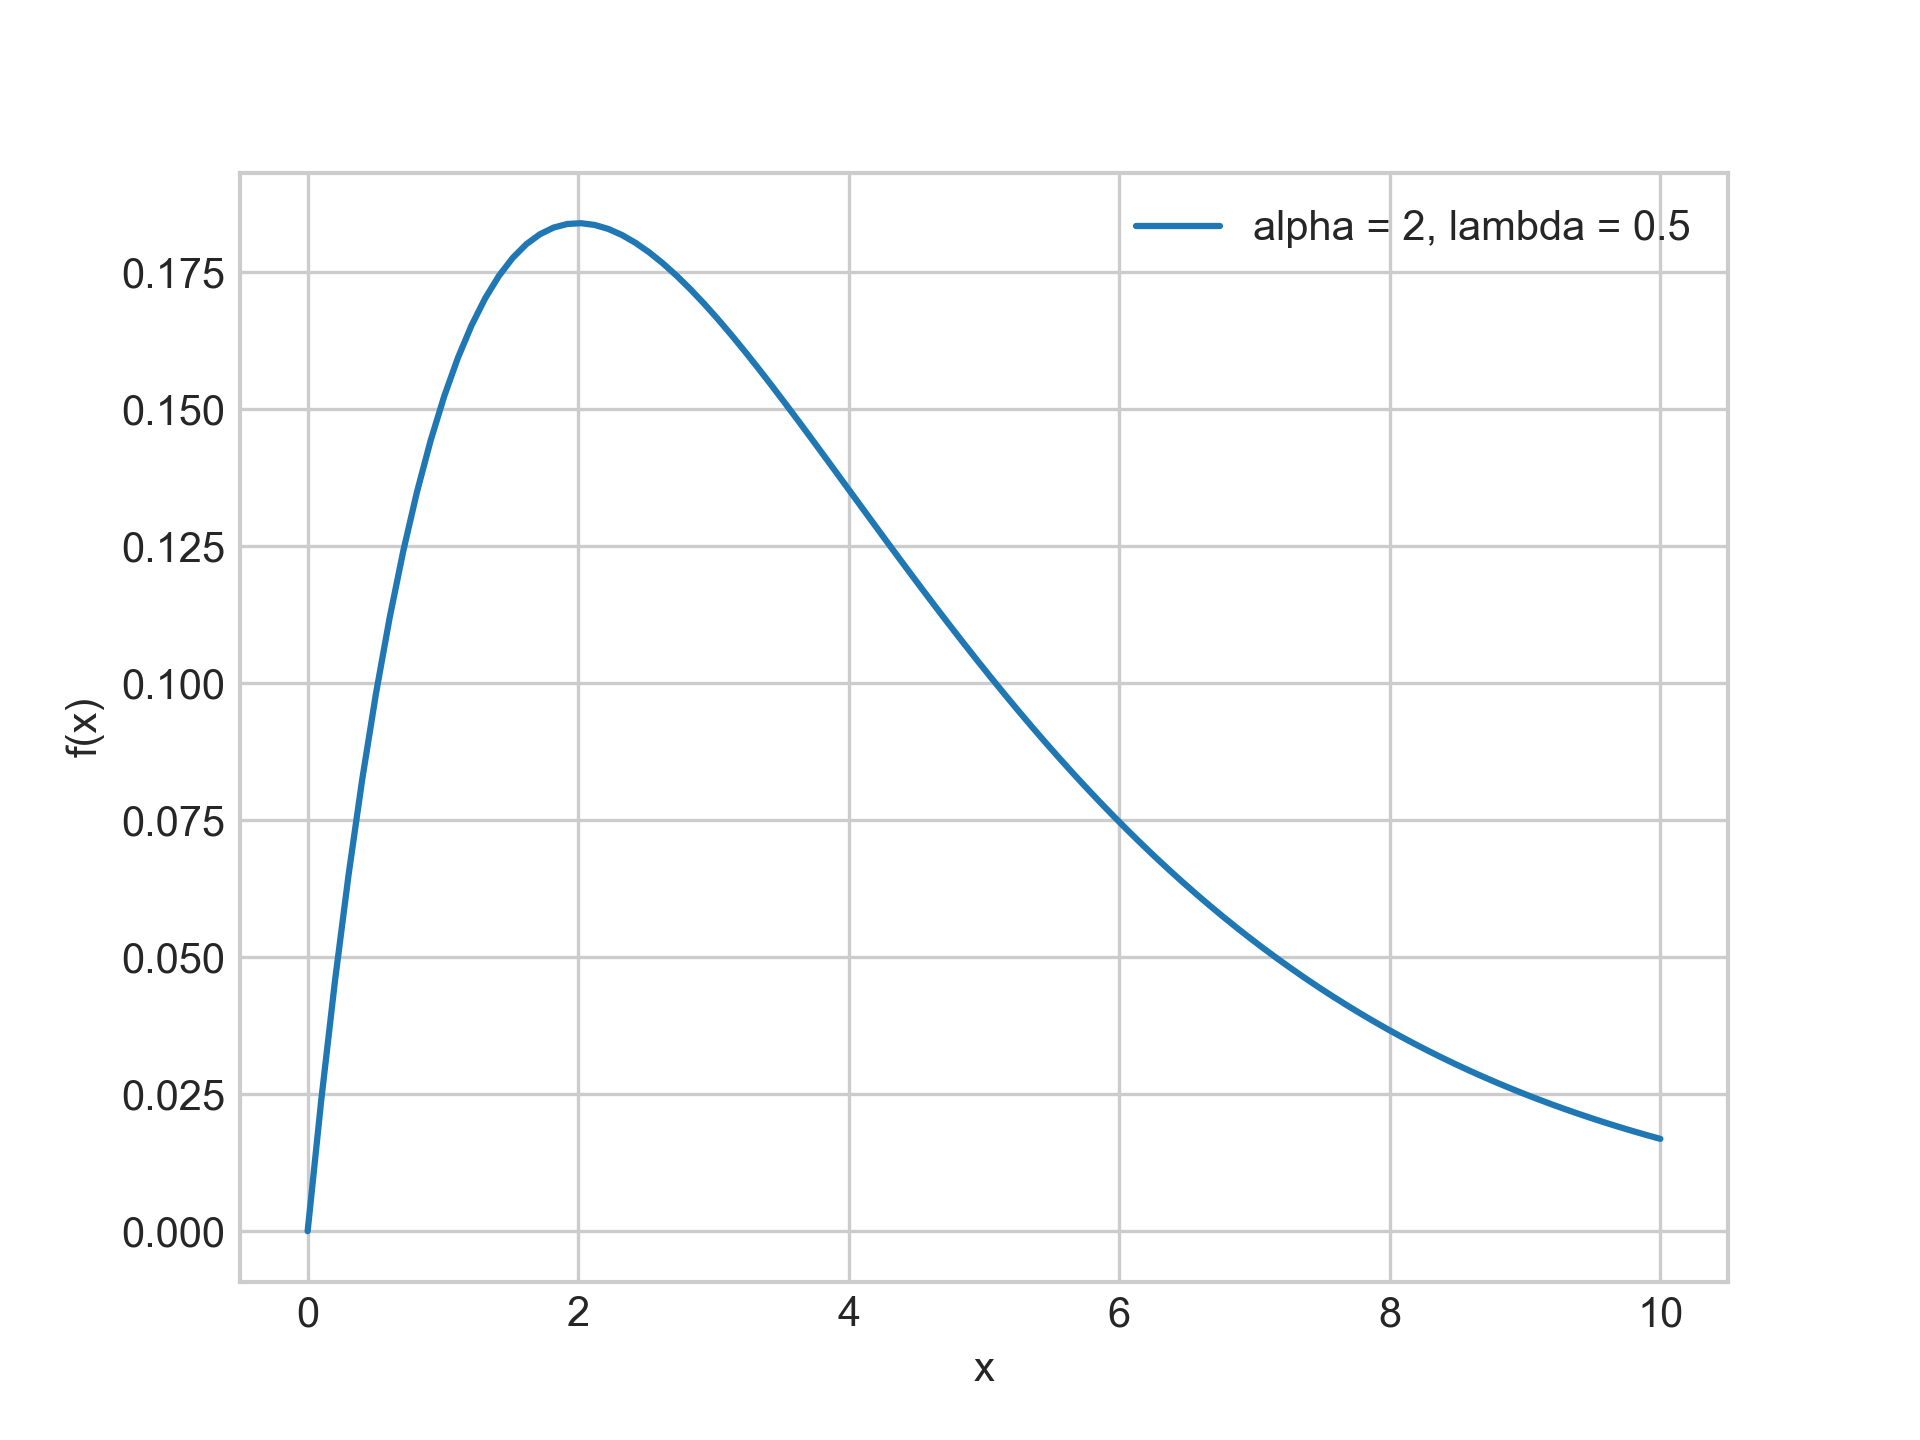
\includegraphics[width=0.4\textwidth]{gamma_pdf.png}
        \captionof{figure}{Probability distribution function of a gamma random variable with $\alpha = 2$ and $\lambda = 0.5$.}
        \label{fig:gamma_pdf}
        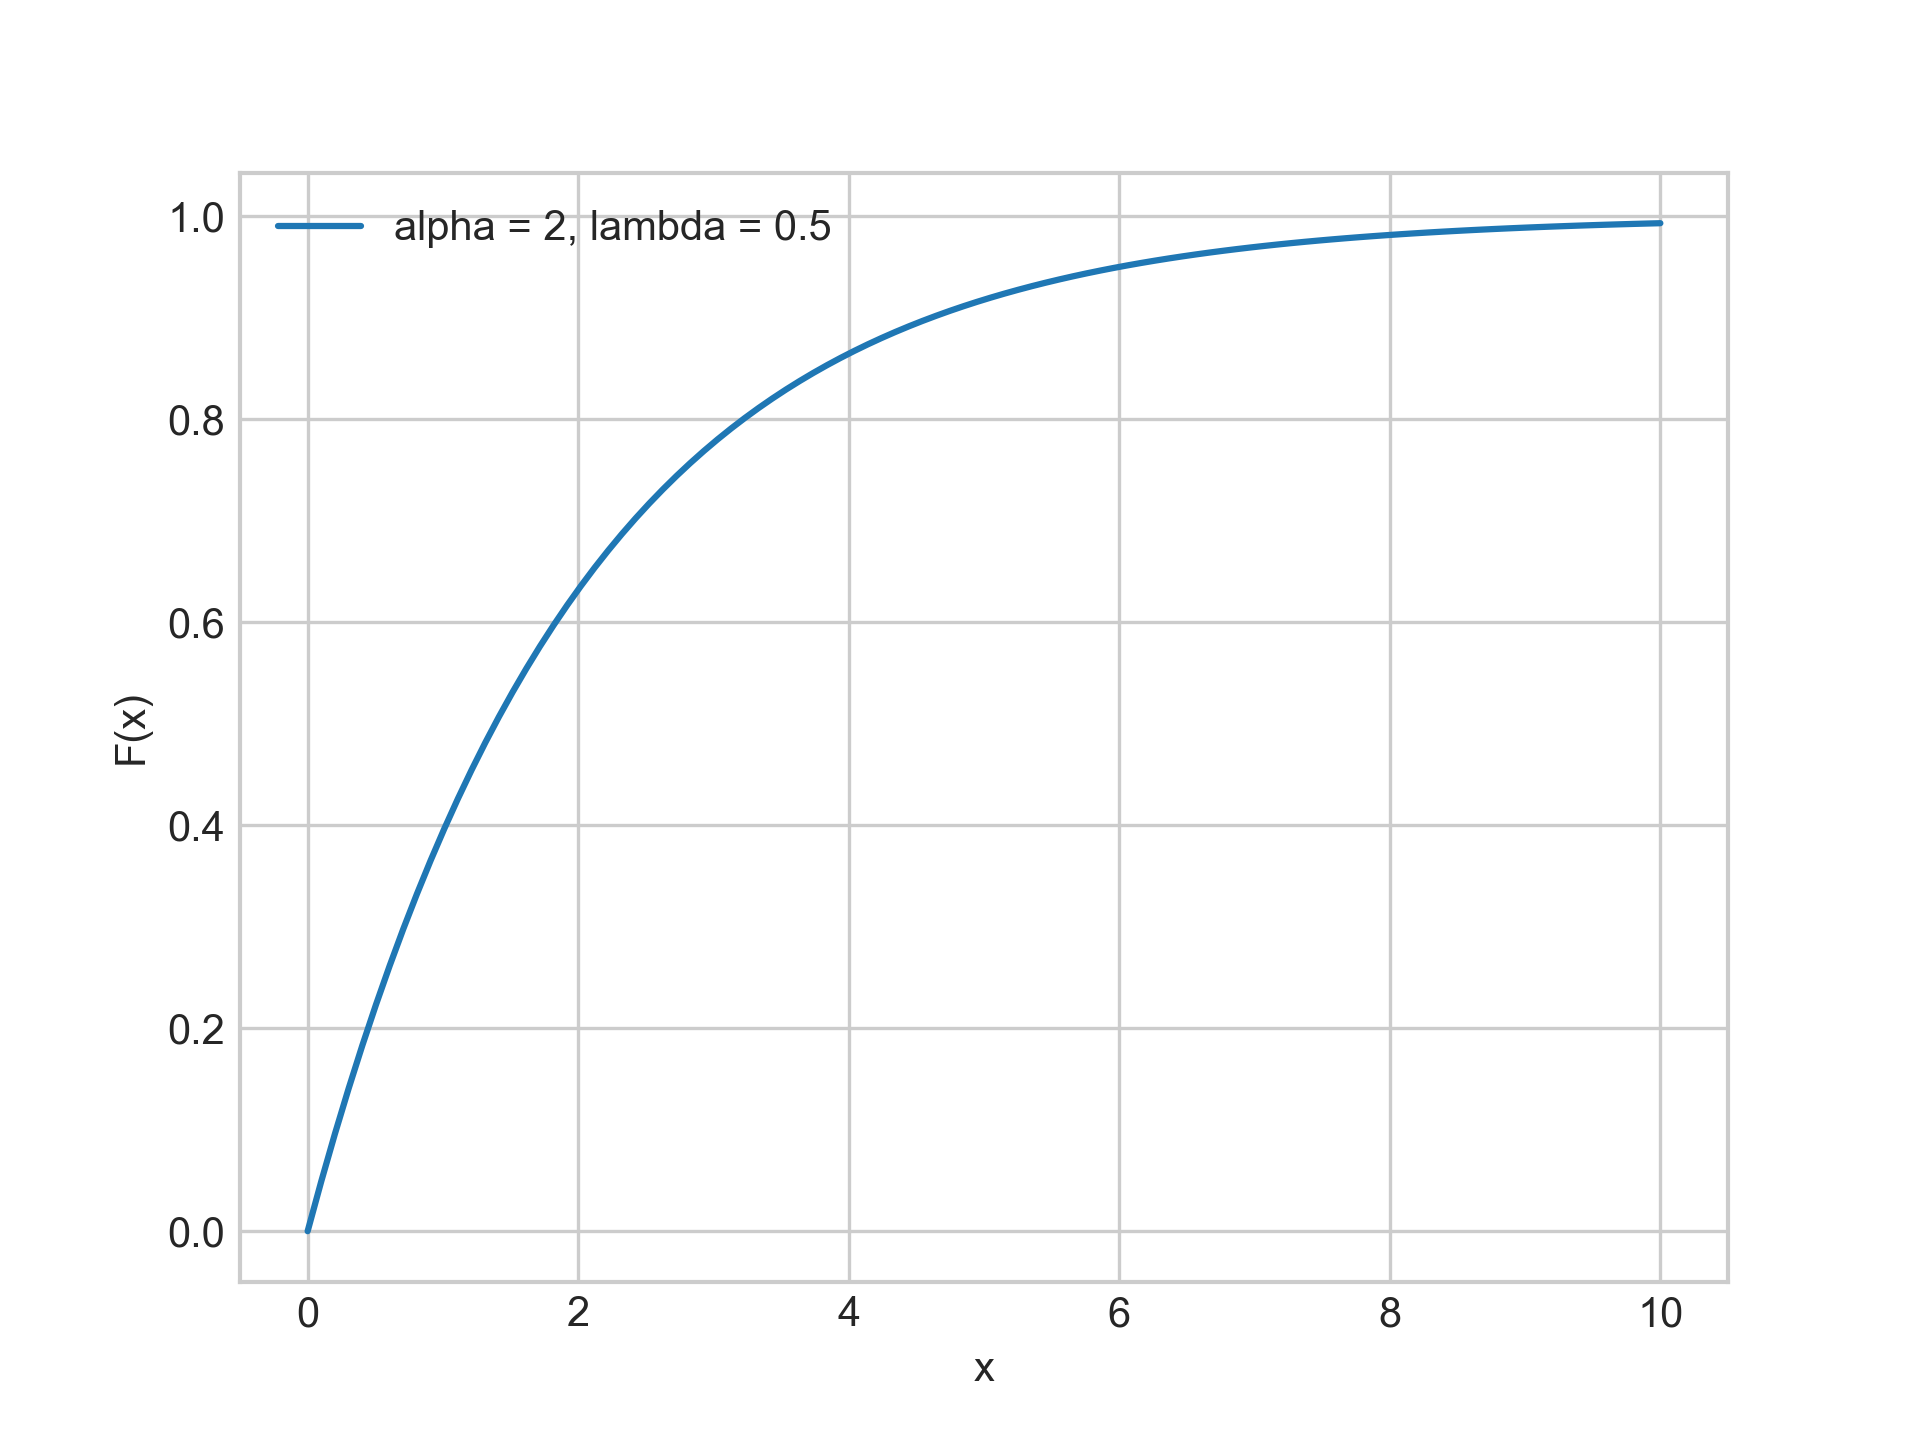
\includegraphics[width=0.4\textwidth]{gamma_cdf.png}
        \captionof{figure}{Cumulative distribution function.}
    \end{center}
}.

\Definition{
The gamma distribution is a probability distribution that models the sum of $n$ exponential random variables.\\
The gamma distribution is characterized by two parameters:
\begin{itemize}
    \item $n$ - the number of exponential random variables.
    \item $\lambda$ - the rate of events occurring in the Poisson process.
\end{itemize}
\[ X \sim \text{Ga}(\alpha, \lambda) \]
\[
f(x) = 
\begin{cases}
    \frac{\lambda^{\alpha}}{\Gamma(\alpha)} x^{\alpha-1} e^{-\lambda x} & x \geq 0 \\
    0 & x < 0
\end{cases}
\]
}{Gamma Distribution}

\Proposition{
The expected value of $X\sim \text{Ga}(\alpha, \lambda)$ is given by:
\[
E[X] = \frac{\alpha}{\lambda}
\]
}{
    \begin{equation}
        \begin{aligned}
            E[X] &= \int_{0}^{+\infty} x f(x) dx = \int_{0}^{+\infty} x \frac{\lambda^{\alpha}}{\Gamma(\alpha)} x^{\alpha-1} e^{-\lambda x} dx \\
                &=  \int_{0}^{+\infty} \frac{\lambda^{\alpha}}{\Gamma(\alpha)} x^{\alpha}e^{-\lambda x}
        \end{aligned}
    \end{equation}
    We can see that this is similar to the integral of the gamma function with $\alpha = \alpha +1$, to make it equal, we need to multiply by $\frac{\lambda}{\lambda}$.
    \begin{equation}
        \begin{aligned}
            E[X] &= \frac{1}{\lambda} \overbrace{\frac{\Gamma(\alpha+1)}{\Gamma(\alpha)}}^{=\alpha \Gamma(\alpha)} \underbrace{
            \int_{0}^{+\infty} \frac{\lambda^{\alpha+1}}{\Gamma(\alpha+1)} x^{\alpha}e^{-\lambda x} dx}_{= 1} \\
            &= \frac{\alpha}{\lambda}
        \end{aligned}
    \end{equation}
}


\section{Uniform Distribution}

If all outcomes in an interval are equally likely, we have a uniform distribution.
Its probability distribution function is given by:
\[
f(x) = \begin{cases}
    \frac{1}{b-a} & a \leq x \leq b \\
    0 & \text{otherwise}
\end{cases}
\]

The cumulative distribution function is:
\[
F(t) = \begin{cases}
    0 & x < a \\
    \frac{t-a}{b-a} & a \leq x \leq b \\
    1 & x > b
\end{cases}
\]

The expected value and variance of a uniform random variable are given by:
\[
E[X] = \frac{a+b}{2} \qquad Var[X] = \frac{(b-a)^2}{12}
\]



% \newpage

% \setchapterabstract{ }
% \chapter{Conditional Probability}
% \vspace{-1.5cm}


% %%%%%%INSERT TOC BELOW 1ST SECTION%%%%%%%%%%%%

% {\chaptoc\noindent\begin{minipage}[inner sep=0,outer sep=0]{0.9\linewidth}\section{Conditional Probability}\end{minipage}}

% \Example{Consider an experiment where a coin is flipped three times. Let the probability of getting heads in each coin flip be $p$.}


% Consider two random variables, \\
% - $X$ representing the probability of getting heads in the $1^{st}$ and $2^{nd}$ coin flips;\\
% - $Y$ representing the probability of getting tails in the $2^{nd}$ and $3^{rd}$ coin flips.
% $$ X \sim \text{Bin}(2, p) \qquad Y \sim \text{Bin}(2, q) \qquad q=1-p $$

% The following matrix represents the distribution of $X$ and $Y$, with the number of heads in the $1^{st}$ and $2^{nd}$ coin flips on the rows and the number of tails in the $2^{nd}$ and $3^{rd}$ coin flips on the columns. The marginal distribution of $X$ and $Y$ are given on the right and bottom of the matrix, respectively.
% \[
% \begin{array}{c|ccc|c}
% & 0 & 1 & 2 & \\
% \hline
% 0 & 0 & pq^2 & q^3 & q^2 \\
% 1 & p^2q & pq & pq^2 & 2pq\\
% 2 & p^2 & p^2q & 0 & p^2\\
% \hline
% & p^2 & 2pq & q^2 &
% \end{array}
% \]


\newpage

\setchapterabstract{In day 6, we discuss the concept of conditional probability distributions in the context of discrete and continuous random variables. We then introduce the concept of sample mean and variance of a set of random variables. Finally, we discuss the concept sequences of random variables and their convergence.}
\chapter{Conditional Probability and Sequences of R.V.s}
\vspace{-1.5cm}

{\chaptoc\noindent\begin{minipage}[inner sep=0,outer sep=0]{0.9\linewidth}\section{Exercise}\end{minipage}}

\[
X \sim \text{Gamma}(\alpha, \lambda) \qquad Y \sim \text{Gamma}(\beta, \lambda)
\]
\[
\begin{cases}
    V = \frac{x}{y} \\
    W = X + Y
\end{cases}
\]
\[
        \begin{cases}
            V = \frac{x}{y} \\
            W = Y(1+V)
        \end{cases}
\]
\[
    \begin{cases}
        X = \frac{VW}{1+V} \\
        Y = \frac{W}{1+V}
    \end{cases}
\]
\[
        J = det \begin{vmatrix}
            \frac{W(1+V)-vw}{(1+V)^2} & \frac{v}{1+v} \\
            -\frac{w}{(1+v)^2} & \frac{1}{1+v}
        \end{vmatrix} = \frac{w}{(1+v)^2}
\]

The density of $X$ and $Y$ is given by:
\[
f_{X, Y}(x, y) = \frac{\lambda^\alpha}{\Gamma(\alpha)} x^{\alpha-1} e^{-\lambda x} \frac{\lambda^\beta}{\Gamma(\beta)} y^{\beta-1} e^{-\lambda y} 
\]
X and Y are two independent random variables, therefore the joint distribution of V and W is given by:
\[
f_{V, W}(v, w) = f_{X, Y}(x, y) \left|J\right| = f_X\left(\frac{vw}{1+v}\right) f_Y\left(\frac{w}{1+v}\right) \frac{w}{(1+v)^2}
\]
\[
f_{V, W}(v, w) = \frac{\lambda^{\alpha+\beta}}{\Gamma(\alpha)\Gamma(\beta)} (\frac{vw}{1+v})^{\alpha-1} e^{-\lambda \frac{vw}{1+v}} (\frac{w}{1+v})^{\beta-1} e^{-\lambda \frac{w}{1+v}} \frac{w}{(1+v)^2}
\]
\[
f_{V, W}(v, w) = \frac{\lambda^{\alpha+\beta}}{\Gamma(\alpha)\Gamma(\beta)} \frac{v^{\alpha-1}}{(1+v)^{\alpha + \beta}} w^{\alpha + \beta-1} e^{-\lambda w} \mathbbm{1}_{(0, +\infty)}(v) \mathbbm{1}_{(0, +\infty)}(w)
\]

If the joint density is the product of two functions, then the two random variables are independent.

The joint density is therefore
\[
f_{V, W}(v, w) = \frac{\gamma^{\alpha+\beta}}{\Gamma(\alpha)\Gamma(\beta)} \frac{v^{\alpha-1}}{(1+v)^{\alpha + \beta}}  \frac{\lambda^{\alpha +\beta}}{(1+v)^(\alpha + \beta)} e^{-\lambda w} \mathbbm{1}_{(0, +\infty)}(v) \mathbbm{1}_{(0, +\infty)}(w)
\]

\section{Conditional Distributions}
\subsection*{Discrete Case}

Consider two random variables $X$ and $Y$ with the following joint distribution:
\[
\begin{array}{c|ccc}
    & 1 & 2 & 3  \\
    \hline
    0 & 0.1 & 0.2 & 0.1 \\
    1 & 0.2 & 0.1 & 0.3
\end{array}
\]

We can calculate the conditional distribution\sn{
    \textbf{Conditional Distribution:} the probability distribution of a random variable, calculated according to the rules of conditional probability after observing the realization of another random variable.
} of $Y$ given $X$:
\[
P(Y = 1 | X = 0) = \frac{P(Y=1, X=0)}{P(X=0)} = \frac{0.1}{0.4}
\]
More in general:
\[
P_{Y|X}(y_i | x_i) = \frac{P_{XY}(y_i, x_i)}{P_{X}(x_i)}
\]
Expected values can be evaluated in the same way:
\[
E(Y|X = 0) = 1 \cdot 0.25 + 2 \cdot 0.5 + 3 \cdot 0.25 = 2
\]
The same can be done for the variance:
\[
Var(Y|X = 0) = E(Y^2|X = 0) - E(Y|X = 0)^2
\]
\[
E(Y^2|X = 0) = 1^2 \cdot 0.25 + 2^2 \cdot 0.5 + 3^2 \cdot 0.25 = 4.5
\]
\[
Var(Y|X = 0) = 4.5 - 2^2 = 0.5
\]

\subsection*{Continuous Case}

\begin{equation*}
    f_{XY}(x,y) = \begin{cases}
        \frac{15}{8}xy^2 \qquad (x,y) \in T \qquad = \frac{15}{8} \mathbbm{1}_{(0,1)}(x) \mathbbm{1}_{(0,2x)}(y) \\
        0 \qquad \text{otherwise}
    \end{cases}
\end{equation*}

Can we construct the conditional distribution of $X$ and $Y$?
In this case, we cannot use the formula $P_{Y|X}(y_i | x_i) = \frac{P_{XY}(y_i, x_i)}{P_{X}(x_i)}$ because the probability of $X$ is zero. We can, however, use the formula for the continuous case:

\[
f_{Y|X}(y|x) = \frac{\frac{15}{8}xy^2\mathbbm{1}_{(0,1)}(x) \mathbbm{1}_{(0,2x)}(y)}{5x^4 \mathbbm{1}_{(0,1)}(x)} = \frac{3}{8}\frac{y^2}{x^3} \mathbbm{1}_{(0,2x)}(y)
\]

We can now calculate the expected value of $Y$ given $X$, as the integral of $y$ times the conditional density of $Y$ given $X$:
\[
E(Y|X = x) = \int_{-\infty}^{+\infty} y f_{Y|X}(y|x) dy = \int_{-\infty}^{+\infty} y \frac{3}{8}\frac{y^2}{x^3} \mathbbm{1}_{(0,2x)}(y) dy
\]
\[
E(Y|X = x) = \int_{0}^{2x} \frac{3}{8} y^3 x^{-3} dy = \frac{3}{8} x^{-3} \frac{y^4}{4} \Big|_{0}^{2x} = \frac{3}{8} x^{-3} \frac{16x^4}{4} = \frac{3}{2}x
\]
The variance can be calculated in the same way:
\[
Var(Y|X = x) = E(Y^2|X = x) - E(Y|X = x)^2
\]
\[
E(Y^2|X = x) = \int_{-\infty}^{+\infty} y^2 f_{Y|X}(y|x) dy = \int_{0}^{2x} \frac{3}{8} y^4 x^{-3} dy
\]
\[
= \frac{3}{8} x^{-3} \frac{y^5}{5} \Big|_{0}^{2x} = \frac{12}{5}x^2
\]
So the variance is:
\[
Var(Y|X = x) = \frac{12}{5}x^2 - \left(\frac{3}{2}x\right)^2 = \frac{3}{20}x^2
\]

\Remark{
If, in the discrete or continuous case, you construct the conditional distribution of $Y$ given $X$, the expected value and variance of $Y$ given $X$ are functions of $X$. This holds true unless $X$ and $Y$ are independent.
}

\Example{
    Let's go back to the previous example:
    \[
    \begin{array}{c|ccc}
        & 1 & 2 & 3  \\
        \hline
        0 & 0.1 & 0.2 & 0.1 \\
        1 & 0.2 & 0.1 & 0.3
    \end{array}
    \]
    We know that $ E(Y|X = 0) = 2 $, what is $ E(Y|X = 1) $?
}

\[
E(Y|X = 1) = 1 \cdot \frac{0.2}{0.6} + 2 \cdot \frac{0.1}{0.6} + 3 \cdot \frac{0.3}{0.6} = \frac{13}{6}
\]

As in the continuous case, the expected value of $Y$ given $X$ is a function of $X$.
\[
E(X|Y = x) = h(x) = \begin{cases}
    2 \qquad x = 0 \\
    \frac{13}{6} \qquad x = 1
\end{cases}
\]

\subsection*{General case}
\[
E(Y|X) = h(X) \leftarrow \text{random variable}
\]
In this case, there is no $X = x$ in the conditional expectation, so we need to calculate the expected value of $Y$ given $X$ as a function of $X$, not of $x$.

So, in the example above:
\[
E(Y|X) = \frac{3}{2}X
\]

\Definition{
    The conditional expectation of $Y$ given $X$ is a random variable $h(X)$. (a function of $X$)\\
    \[
    E(Y|X) = h(X)
    \]
    \textbf{Properties}:\\
        - $E(E(Y|X)) = E(Y)$ (Tower Property) \\
        - $E(Yg(X)|X) = g(X)E(Y|X)$ \\
        - $Var(Y|X)$ is a r.v. \\
        - $Var(Y) = Var(E(Y|X)) + E(Var(Y|X))$
}{Conditional Expectation}


\Example{
    Suppose that $Y$ is a random variable ``duration of battery", and $X$ is the r.v. ``percentage of an element"
    \[
    X \sim \text{Uniform}(1, 3) \qquad (Y|X = x) \sim \text{Exp}(\lambda = x)
    \]
    What is the average duration of the battery? i.e. $E(Y)$
}

\[
E(Y|X=x)=\frac{1}{x} \qquad E(Y|X) = \frac{1}{X}
\]

Therefore, we can use the Tower Property:
\[
E(Y) = E(E(Y|X)) = E\left[\frac{1}{X}\right] = \int_{1}^{3} \frac{1}{x} \frac{1}{2} dx = \frac{1}{2} \int_{1}^{3} \frac{1}{x} dx = \frac{1}{2} \ln(3)
\]

\Example{
    The duration of a call is:
    \(
    T_1 \sim \text{Exp}(\lambda = \frac{1}{2})
    \) \\
    The number of calls is:
    \(
    N \sim \text{Poisson}(\lambda = 60)
    \)\\
    The total time spent on calls is therefore:
    \[
    Y = \sum_{i=1}^{N} T_i
    \] \\
    What is the expected value and variance of the total time spent on calls?
}

\[
(Y|N = n) = \sum_{i=1}^{n} T_i \sim \text{Gamma}(n, \frac{1}{2})
\]

\[
E(Y|N=n) = E(Ga(n, \frac{1}{2})) = \frac{n}{\lambda} = 2n
\]
\[
E(Y) = E(E(Y|N)) = E(2N) = 2E(N) = 2 \cdot 60 = 120
\]
Calculating the variance:
\[
Var(Y|N=n) = n \cdot \frac{1}{\lambda^2} = 4n
\]
\[
Var(Y) = Var(E(Y|N)) + E(Var(Y|N))
\]
\[
Var(Y) = Var(2N) + E(4N) = 4Var(N) + 4E(N) = 4 \cdot 60 + 4 \cdot 60 = 480
\]

\Example{
    Suppose $X_1, \ldots , X_n$ are independent and identically distributed random variables with $X_n \sim \text{Bern}(p)$.\\
    Let $Y = \sum_{i=1}^{n} X_i$. \\
    What is $E(X_1 | Y)$?
}

The distribution of $Y$ is a binomial: $Y \sim \text{Bin}(n, p)$.
\[
E(X_1 | Y = k) = 0 \cdot P(X_1 = 0 | Y = k) + 1 \cdot P(X_1 = 1 | Y = k)
\]
\[
E(X_1 | Y = k) = P(X_1 = 1 | Y = k) = \frac{P(X_1 = 1, Y = k)}{P(Y = k)}
\]
The possible values of $k$ are $0, 1, \ldots , n$, so:
\[
    E(X_1 | Y = k) = \begin{cases}
        0 \qquad k = 0 \\
        ? \qquad k = 1, \ldots , n
    \end{cases}
\]
We can rewrite the conditional expectation as:
\[
E\left(X_1 | \sum_{i=1}^{n} X_i = k\right) = \frac{P(X_1 = 1, \sum_{i=1}^{n} X_i = k)}{P(\sum_{i=1}^{n} X_i = k)}
\]
The two events in the numerator are not independent, so we have to rewrite it to solve the problem.
The probability of $X_1 = 1$ and $\sum_{i=1}^{n} X_i = k$ is the same as the probability of $X_1 = 1$ and $X_2 + \ldots + X_n = k-1$:
\[
P(X_1 = 1, \sum_{i=1}^{n} X_i = k) = \frac{P(X_1 = 1, \sum_{i=2}^{n} X_i = k-1)}{P(\sum_{i=1}^{n} X_i = k)}
\]
\[
= \frac{P(X_1 = 1)P(\sum_{i=2}^{n} X_i = k-1)}{P(\sum_{i=1}^{n} X_i = k)} = \frac{p\cdot \binom{n-1}{k-1}p^{k-1}q^{n-k}}{\binom{n}{k}p^kq^{n-k}}
\]
\[
= \frac{\binom{n-1}{k-1}}{\binom{n}{k}} = \frac{\frac{(n-1)!}{(k-1)!(n-k)!}}{\frac{n!}{k!(n-k)!}} = \frac{k}{n}
\]
The final result is therefore:
\[    
E(X_1 | Y = k) = \begin{cases}
    0 \qquad k = 0 \\
    \frac{k}{n} \qquad k = 1, \ldots , n
\end{cases}
= \frac{k}{n}
\]
Therefore:
\[
E(X_1 | Y) = \frac{Y}{n}
\]

\section{Sample Mean and Variance}

Take $X_1, \ldots , X_n$ i.i.d. We can define the sample mean $\bar{X} = \frac{1}{n} \sum_{i=1}^{n} X_i$.

Defining $m = E(X_1)$, we can calculate the expected value of the sample mean:

\[
E(\bar{X}) = E\left(\frac{1}{n} \sum_{i=1}^{n} X_i\right) = \frac{1}{n} \sum_{i=1}^{n} E(X_i) = \frac{1}{n} \cdot n \cdot m = m
\]

With the variance of $X_1$ defined as $v$, we can calculate the variance of the sample mean:

\[
Var(\bar{X}) = Var\left(\frac{1}{n} \sum_{i=1}^{n} X_i\right) = \frac{1}{n^2} \sum_{i=1}^{n} Var(X_i) = \frac{1}{n^2} \cdot n \cdot v = \frac{v}{n}
\]

This holds true for any sampling distribution.

\subsection*{Sample Variance}

The sample variance is defined differently, depending on wether $m$ is known or not.

\textbf{If $m$ is known}, the sample variance is:
\[
S_0^2 = \frac{1}{n} \sum_{i=1}^{n} (X_i - m)^2 = \frac{1}{n} \sum_{i=1}^{n} X_i^2 - 2m \sum_{i=1}^{n} X_i + n m^2
\]

The expected value of the sample variance is $E(S_0^2) = v$.

\textbf{If $m$ is unknown}, the sample variance is:

\[
S_n^2 = \frac{1}{n-1} \sum_{i=1}^{n} (X_i - \bar{X_n})^2
\]
This can be rewritten as:
\[
S_n^2 = \frac{1}{n-1} \left[\sum_{i=1}^{n} X_i^2 - \underbrace{2\bar{X_n} \sum_{i=1}^{n} X_i}_{=2\bar{X}_n^2} + n \bar{X_n}^2\right]
\]
\[
S_n^2 = \frac{1}{n-1} \left[\sum_{i=1}^{n} X_i^2 - n \bar{X_n}^2\right]
\]

\subsection*{Case of a Normal Distribution}

Take $X_1, \ldots , X_n$ i.i.d. with $X_i \sim \text{N}(\mu, \sigma^2)$.
Then the sample mean $\bar{X}_n = \frac{1}{n} \sum_{i=1}^{n} X_i$ is normally distributed with:
$\bar{X}_n \sim \text{N}(\mu, \frac{\sigma^2}{n})$.

The sample variance in the case where $m$ is known is distributed as:
\[
\frac{n S_0^2}{\sigma^2} \sim \chi^2(n)
\]

In the case where $m$ is unknown, the sample variance is distributed as:
\[
\frac{(n-1) S_n^2}{\sigma^2} \sim \chi^2(n-1)
\]

\section{Sequence of R.V.s}

\Definition{
In a sequence of real numbers $a_1, a_2, \ldots , a_n$, the limit is defined as:
\[ 
\lim_{n \to \infty} a_n = L \in \mathbb{R} \quad \forall \epsilon > 0 \quad \exists n_\epsilon \in \mathbb{N} \quad | \quad \forall n \geq n_\epsilon \implies  |a_n - L| < \epsilon
\]
}{Limit of a Sequence}

Intuitively, the limit exists if there exists an $n$ large enough so that after that $n$ all the terms are within $\epsilon$ distance of the limit. ($\text{dist}(a_n, L) < \epsilon$)

Limits can be defined in spaces other than $\mathbb{R}$, as long as there is a way to define the distance between two elements.

\textbf{Sequence of Random Variables}

Take a sequence of random variables $X_1, X_2, \ldots , X_n, \ldots$.
Suppose that all the random variables are defined on the same probability space $(\Omega, \mathcal{A}, P)$.

\Definition{
    We say that $X_n \to Y$ surely if:
    \[
    \forall \omega \in \Omega \quad X_n(\omega) \to Y(\omega)
    \]
}{Sure Convergence}

In other words, for every sequence of outcomes $X_n(\omega)$, the limit of the sequence is $X(\omega)$.

This definition is very strong, and is not very useful in practice.

\Definition{
    We say that $X_n \to Y$ almost surely if:
    \[
    P(\{\omega \in \Omega | X_n(\omega) \to Y(\omega)\}) = 1
    \]
}{Almost Sure Convergence}

In other words, the set of outcomes for which the sequence of random variables converges to the limit has probability 1.

Property:
\[
g: \mathbb{R} \to \mathbb{R} \quad \text{continuous} \quad \implies \quad g(X_n) \to g(Y) \quad \text{almost surely}
\]

\Definition{
    We say that $X_n \to Y$ in probability if:
    \[
    \forall \epsilon > 0 \quad \lim_{n \to \infty} P(|X_n - Y| < \epsilon) = 1
    \]
}{Convergence in Probability}

In other words, the probability that the distance between $X_n$ and $Y$ is less than $\epsilon$ converges to 1 as $n$ goes to infinity.

\Definition{
    We say that $X_n \to Y$ in mean of order $k \geq 1$ if:
    \[
    E(|X_n - Y|^k) \to 0
    \]
}{Convergence in Mean of Order $k$}

\Definition{
    We say that $X_n \to Y$ in quadratic mean if:
    \[
    E(|X_n - Y|^2) \to 0
    \]
}{Convergence in Quadratic Mean}


From a sequence of random variables, we can define the sequence of sample means:
\[
\bar{X_1} = X_1 \quad \bar{X_2} = \frac{X_1 + X_2}{2} \quad \bar{X_3} = \frac{X_1 + X_2 + X_3}{3} \quad \ldots
\]
\[
\bar{X}_n = \frac{1}{n} \sum_{i=1}^{n} X_i
\]

We can demonstrate that the sample mean converges to the expected value of the random variable:

\[
Var(\bar{X}_n) = \frac{1}{n^2} \sum_{i=1}^{n} Var(X_i) = \frac{1}{n^2} \cdot n \cdot v = \frac{v}{n}
\]
\[
E(|\bar{X}_n - m|^2) = Var(\bar{X}_n) = \frac{v}{n} \to 0
\]

\Definition{
    If $X_1, X_2, \ldots , X_n$ are i.i.d. with $E(X_i) = m$ and $Var(X_i) = v$, then:
    \[
    \bar{X}_n \to m \quad \text{almost surely}
    \]
}{Strong Law of Large Numbers}

If $X_n \to Y$ almost surely, then $X_n \to Y$ in probability. The converse is not true.
\[
X_n \to Y \text{ almost surely} \quad \underset{\nLeftarrow}{\Rightarrow} \quad X_n \to Y \text{ in probability}
\]

Moreover, if $X_n \to Y$ in order $k$, then $X_n \to Y$ in probability. The converse is again not true.
\[
X_n \to Y \text{ in order } k \quad \underset{\nLeftarrow}{\Rightarrow} \quad X_n \to Y \text{ in probability}
\]

\subsection*{Convergence in Distribution}

\Definition{
    We say that $X_n \to Y$ in distribution if:
    \[
    F_{X_n}(t) \to F_Y(t) \quad \forall t \quad \text{where} \quad F_{Y} \quad \text{is continuous}
    \]
}{Convergence in Distribution}

Convergence in distribution is a weaker form of convergence than other forms of convergence.
Link between convergence in distribution and convergence in probability:
\[
X_n \to Y \text{ in probability} \quad \Rightarrow \quad X_n \to Y \text{ in distribution}
\]

The converse is generally not true. However, if $Y$ is a constant, then the two forms of convergence are equivalent.

\[
X_n \to y \in \mathbb{R} \text{ in distribution} \quad \Leftrightarrow \quad X_n \to y \in \mathbb{R} \text{ in probability}
\]

\Example{
    Take a sequence of i.i.d. random variables $X_1, X_2, \ldots , X_n, \ldots$ with:
    \[ 
    X_i \sim \text{Unif}(0,1)
    \]
    We take the sequence $Y_n = \min(X_1, \ldots , X_n)$.
    What is the limit of $Y_n$?
}

Recall that if $V_n = \min(X_1, \ldots , X_n)$, then $F_{V_n}(t) = 1- [1-F_x(t)]^n.$ 

Since the distribution function of $X$ is:
\[
F_X(t) = \begin{cases}
    0 \qquad t < 0 \\
    t \qquad 0 \leq t \leq 1 \\
    1 \qquad t > 1
\end{cases}
\]

The distribution function of $V_n$ is:
\[
F_{V_n}(t) = \begin{cases}
    0 \qquad t < 0 \\
    1 - (1-t)^n \qquad 0 \leq t \leq 1 \\
    1 \qquad t > 1
\end{cases}
\]

For the convergence in distribution, we need to calculate the limit of $F_{V_n}(t)$ as $n$ goes to infinity:
\[
\lim_{n \to \infty} F_{V_n}(t) = \begin{cases}
    0 \qquad t \leq 0 \\
    1 \qquad t > 0
\end{cases}
\]

This is not the distribution function of any random variable, because it has a jump at 0, and in that jump the value is continuous from the left but not from the right.

This is the distribution of a discrete random variable, as it is not continuous but piecewise constant.
From the definition oif the limit of a sequence of random variables, we can define the limit of $F_{V_n}(t)$ as:
\[
F_Y(t) = \begin{cases}
    0 \qquad t < 0 \\
    1 \qquad t \geq 0
\end{cases}
\]

Which is the distribution function of a random variable $Y$ that is equal to 0 with probability 1.

\section{Central Limit Theorem}
\Definition{
    Let $X_1, \ldots, X_n$ be i.i.d random variables with $m = E(X_i)$ and $v = Var(X_i)$.\\
    \[
    \mathbb(P)\left(\frac{\bar{X}_n - m}{\sqrt{\frac{v}{n}}} \leq t\right) \to \Phi(t) \quad \text{as} \quad n \to +\infty
    \]
    or
    \[
    \frac{\bar{X}_n - m}{\sqrt{\frac{v}{n}}} \to \text{N}(0,1) \quad \text{in distribution}
    \]
    For this to hold, we have to assume that the random variables have finite mean and variance. In other words, $E(X_i^2) < +\infty$.
}{Central Limit Theorem}

In other words, if $n$ is ``large enough", then the distribution of the sample mean is approximately normal with $\bar{X_n} \approx N(m, \frac{v}{n})$.

If we multiply by $n$, we get:
\[
\sum_{i=1}^{n} X_i \approx N(nm, nv)
\]

Take $Y \sim \text{Bin}(n,p)$, then if $n$ is large enough and $p$ is not too close to 0 or 1, then $Y \approx N(np, npq)$.

With a binomial distribution $Y \sim \text{Bin}(n,p)$, if $n \to +\infty$ and $p \to 0$ such that $np \to \lambda$, then $Y \approx \text{Po}(\lambda)$. In other words, $X_n \to P(\lambda)$ in distribution.

Poisson random variables are also approximately normal if $\lambda$ is large enough.\sn{The Poisson distribution with parameter $\lambda$ is the sum of $\lambda$ Poisson random variables with parameter 1.}

In the case of Gamma distributions $Y\sim \text{Ga}(\alpha, \lambda)$, if $\alpha$ is large enough, then $Y \approx N(\alpha/\lambda, \alpha/\lambda^2)$.\sn{The Gamma distribution with parameters $\alpha$ and $\lambda$ is the sum of $\alpha$ exponential random variables with parameter $\lambda$.}

For a Chi-squared distribution with $n$ degrees of freedom, if $n$ is large enough, then $X \approx N(n, 2n)$.\sn{The Chi-squared distribution with $n$ degrees of freedom is the sum of $n$ standard normal random variables squared ($\chi^2$ with 1 d.f.).}

\Definition{
Let $X_n \to X$ in distribution. If $Y_n \to Y$ in probability, then:
\[
X_n + Y_n \to X + Y \quad \text{in distribution}
\]
\[
X_n \cdot Y_n \to X \cdot Y \quad \text{in distribution}
\]
$\forall n  \quad P(Y_n = 0) = 0$ and $y \neq 0$.
}{Slutsky's Theorem}

\textbf{Sampling from a Normal Distribution}

Take $X_1, X_2, \ldots , X_n$ i.i.d. with $X_i \sim N(\mu, \sigma^2)$.
\[
\frac{\bar{X}_n - \mu}{\sqrt{\frac{S_n^2}{n}}} = \underbrace{\frac{\bar{X}_n - \mu}{\sqrt{\frac{\sigma^2}{n}}}}_{\sim N(0,1)} \underbrace{\sqrt{\frac{\sigma^2}{S_n^2}}}_{\to 1} \to Z \sim N(0,1) \text{in distribution}
\]
Therefore, the distribution is approximately $N(0,1)$.

\textbf{Sampling not from a Normal Distribution}
If $m = E(X_i)$ and $v = Var(X_i)$, then:
\[
\frac{\bar{X}_n - \mu}{\sqrt{\frac{S_n^2}{n}}} = \underbrace{\frac{\bar{X}_n - \mu}{\sqrt{\frac{v}{n}}}}_{\sim Z} \underbrace{\sqrt{\frac{v}{S_n^2}}}_{\to 1} \to Z \sim N(0,1) \text{in distribution}
\]

